\chapter{Dataset}
In questo capitolo viene analizzato il dataset. Viene quindi spiegato
da dove è stato preso il dataset, descritte le covariate e viene
effettuata un'analisi esplorativa.

\section{Acquisizione del dataset}
Il dataset completo contenente sia le informazioni sui singoli
musicali che le etichette associate ad ogni istanza non è
disponibile da una sola sorgente. Pertanto abbiamo ottenuto le
informazioni necessarie da diversi sorgenti per poi integrarle in un
unico dataset.

\subsection{Dataset spotify - Kaggle}
Per quanto riguarda i brani con le relative informazioni e
caratteristiche del brano, Spotify mette a disposizone un'API da cui
si possono ottenere questi dati.

Con questa tecnica sono stati ottenuti i dati relativi ai brani, un utente ha quindi caricato il dataset sul sito \href{https://www.kaggle.com/}{kaggle.com}. Il dataset è disponibile su kaggle all'url indicato\footnote{\textbf{Dataset Spotify}: \href
	{https://www.kaggle.com/yamaerenay/spotify-dataset-19212020-160k-tracks}
	{https://www.kaggle.com/yamaerenay/spotify-dataset-19212020-160k-tracks}.}.

Il dataset contenente queste informazioni è il file: \verb|data/raw/to_integrate/data.csv|.
\subsection{Premi canzoni - Wikipedia}
Le informazioni riguardo i premi delle canzoni, ovvero le varie certificazioni vinte, sono disponibili su \href{https://it.wikipedia.org//}{wikipedia.org}. Questa informazione costituisce di fatto l'etichetta per classificare ogni brano musicale come di successo o non di successo..

Nello specifico siamo interessati a:
\begin{itemize}
	\item Singoli certificati oro
	\item Singoli certificati platino
	\begin{enumerate}
		\item Singoli certificati 1 volta platino
		\item Singoli certificati 2 volte platino
		\item ...
		\item Singoli certificati N volte platino
	\end{enumerate}
\end{itemize}

Inoltre le varie certificazioni dei singoli vengono considerati in base al paese. I paesi da noi presi in considerazione sono:
\begin{itemize}
	\item Italia
	\item Australia
	\item Stati Uniti d'America
	\item Regno Unito
	\item Canda
	\item Danimarca
\end{itemize}
Si noti come una certificazione può essere consegnata in diversi paesi alla stessa canzone.

\subsubsection{Certificazioni disco d'oro}
Per quanto riguarda i dischi d'oro, facciamo riferimento a questa pagina su wikipedia \footnote{\textbf{Disco d'oro per stato}:\\
	\href
	{https://it.wikipedia.org/wiki/Categoria:Singoli_certificati_oro_per_stato}
	{https://it.wikipedia.org/wiki/Categoria:Singoli\_certificati\_oro\_per\_stato}.}.
Fissato quindi uno stato (ad esempio l'Italia) è possibile visualizzare la pagina contenente la lista dei singoli che hanno vinto quel particolare premio. La lista è un elenco di url che puntano alla pagina wikipedia della canzone, un esempio a questo url\footnote{\textbf{Singoli certificati disco d'oro in Italia}:\\
	\href
	{https://it.wikipedia.org/wiki/Categoria:Singoli\_certificati\_disco\_d\%27oro_in_Italia}
	{https://it.wikipedia.org/wiki/Categoria:Singoli\_certificati\_disco\_d\%27oro\_in\_Italia}.}.

\subsubsection{Certificazioni disco di platino}
Ragionamento analogo viene fatto per i dischi di platino, con l'unica differenza che la pagina è questa\footnote{\textbf{Singoli certificati disco di platino per stato}:\\
	\href
	{https://it.wikipedia.org/wiki/Categoria:Singoli_certificati_platino_per_stato}
	{https://it.wikipedia.org/wiki/Categoria:Singoli\_certificati\_platino\_per\_stato}.}, inoltre
dal momento che i singoli posso vincere più volte un disco di platino, si considerano non solo i singoli che hanno vinto una volta il discho di platino ma anche quelli che l'hanno vinto N volte.

\subsubsection{Scraping}
Ottenuti quindi i puntatori alle canzoni certificate, è possibile accedere alla pagina wikipedia del singolo, la quale contiene una tabella riassuntiva della canzone. Un esempio di tabella viene mostrato nella Figura \ref{fig:wiki_table}.
\begin{figure}[H]
	\centering
	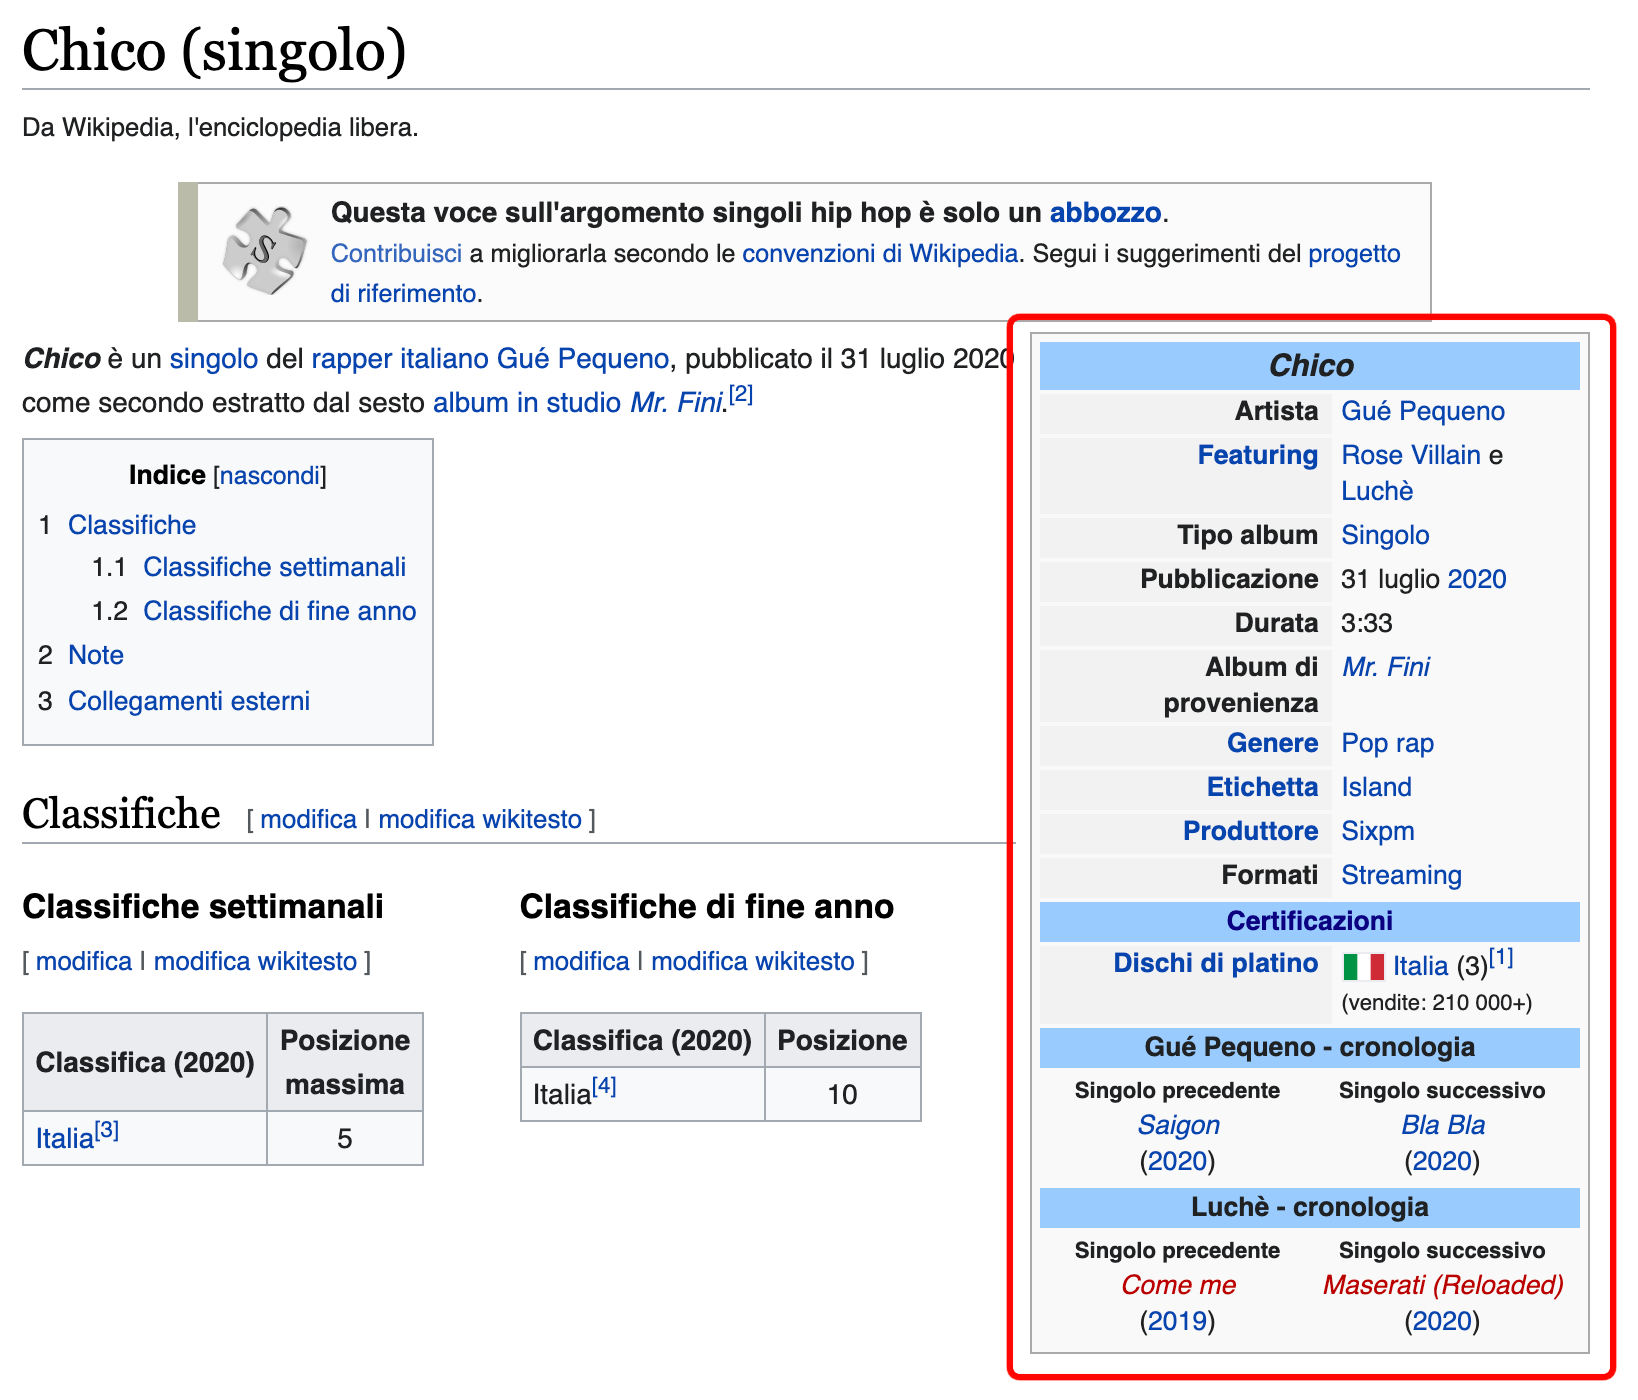
\includegraphics[width=12cm]{assets/wikipedia-table.png}
	\caption{Esempio di tabella per un singolo musicale su wikipedia}
	\label{fig:wiki_table}
\end{figure}

Viene quindi creato uno script per effettuare scraping delle tabelle, il codice è nella directory\\ \verb|scraping/wikipedia_songs_scraper.py|.

Successivamente si integrano le informazioni dei diversi stati, e tipi di certificazione vinti. Il risultato di questa operazione è il file \verb|data/raw/to_integrate/awards_cleaned.csv|.

\section{Descrizione del dataset}
In questa sezione vengono elencate e descritte le features del
dataset. Trattandosi di un problema supervisionato, ad ogni istanza
viene associata la corretta etichetta, ovvero la classe positiva per i
brani musicali che hanno vinto un premio e classe negativa per i brani
che non hanno vinto un premio.
\subsection{Spotify}
\label{sec:descrizione_spotify}
Di seguito viene descritto il dataset proveniente da kaggle, quindi quello contenente le informazioni dei brani.

\begin{center}
	
	\resizebox{\textwidth}{!}{
		\begin{tabular}[H]{ |l|l|l| }
			\hline
	
			\multicolumn{1}{ |c }{\textbf{ATTRIBUTO}} &
			\multicolumn{1}{ c }{\textbf{DESCRIZIONE}} &
			\multicolumn{1}{ c| }{ \textbf{TIPO}} \\
			
			\hline
			\hline
			
			id & 
			Identificativo della canzone (generato da spotify) &
			Intero\\
			
			name & 
			Titolo della canzone &
			Stringa\\
			
			artists & 
			Lista degli artisti che compaiono nel brano &
			Stringa\\
			
			year & 
			Anno del brano &
			Intero\\
			
			duration\_ms & 
			Durata della traccia in millisecondi &
			Intero\\
			
			acousticness & 
			Metrica riguardante quanto un brano risulta "acustico" &
			Float [0, 1]\\
			
			danceability & 
			Metrica riguardante quanto una traccia è ballabile &
			Float [0, 1]\\
			
			energy & 
			Energia del brano &
			Float [0, 1]\\
			
			instrumentalness & 
			Contenuto relativo di strumenti musicali nella traccia&
			Float [0, 1]\\
			
			valence & 
			Metrica riguardante la "positività" della traccia &
			Intero\\
			
			liveness & 
			Durata relativa della traccia suonata in una performance dal vivo &
			Float [0, 1]\\
			
			loudness & 
			Rumorosità della traccia in decibel (dB) &
			Float [-60, 0]\\
			
			release\_date & 
			Anno di rilascio del brano&
			Intero\\
			
			speechiness & 
			Contenuto relativo di voce umana nella traccia &
			Float [0, 1]\\
			
			tempo & 
			BPM della traccia &
			Float\\
			
			key & 
			Scala musicale utilizzata &
			Factor \{0, 1, ..., 11\}\\
			
			mode & 
			Indica se la traccia parte con una progressione armonica &
			Booleano\\
			
			explicit & 
			Indica se la traccia è esplicita oppure no (linguaggio volgare) &
			Booleano\\
			
			popularity & 
			Popolarità della traccia &
			Float [0, 100]\\
			
			\hline
			
		\end{tabular}
	}
\end{center}

\subsection{Premi}
Si noti come la distinzione tra tipo di premio vinto e lo stato in cui
è stata ottenuta la certificazione per uno specifico brano, viene
fatta solo nel contesto della attivitá di scraping, in quanto i brani
sono così rappresentati sul sito di wikipedia. Tuttavia da questo
punto in poi non verrà più tenuto conto di questa informazione,
infatti un singolo verrà considerato come\textbf{ vincitore di un
  premio} (quindi di successo) oppure come \textbf{non vincitore di
  un premio} (non di successo). I brani musicali vincitori di un premio appartengono alla classe positiva, viceversa quelli che non hanno vinto un premio alla classe negativa.

Il risultato dello scraping della tabella di wikipedia è il seguente:

\begin{center}
	
	\resizebox{\textwidth}{!}{
		\begin{tabular}[H]{ |l|l|l| }
			\hline
			
			\multicolumn{1}{ |c }{\textbf{ATTRIBUTO}} &
			\multicolumn{1}{ c }{\textbf{DESCRIZIONE}} &
			\multicolumn{1}{ c| }{ \textbf{TIPO}} \\
			
			\hline
			\hline
			
			title & 
			Titolo della canzone &
			Stringa\\
			
			artists & 
			Artisti presenti nela traccia &
			Stringa\\
			
			date & 
			Data di rilascio della traccia &
			Data\\
			
			genre & 
			Genere musicale del brano&
			Stringa\\
			
			award & 
			Premio vinto dal singolo&
			Stringa \{Oro, 1\_platino, 2\_platino, ...\}\\
			
			nation & 
			Paese in cui è stato vinto il premio&
			Stringa (Sigla del paese)\\
			\hline
			
		\end{tabular}
	}
\end{center}

\section{Data integration}
Date queste due sorgenti dati, è necessario integrare i dati allo
scopo di avere un dataset etichettato, le label saranno appunto se un
brano musicale ha vinto un premio (quindi è di successo) oppure no.

La strategia di entity resolution adottata è considerare un singolo
musicale come una singola entità basandosi sul titolo e gli artisti
di una canzone. Se il nome del brano musicale è lo stesso e gli
artisti coincidono, allora il brano è il medesimo.

\subsection{Record linkage con MongoDB}
A questo scopo i due dataset vengono importati in mongoDB, ogni
istanza è rappresentata da un documento. Per la fase di record linkage
vengono effettuati i seguenti passi:

\begin{enumerate}
	\item Import dei dataset in mongodb, inizialmente in due collezioni diverse.
	\item Normalizzazione dei dati, i campi di join vengono trasformati in lowercase.
	\item Creazione indici.
	\item Entrambe le collezioni hanno il campo "artisti" il quale consiste in una stringa contenente la lista degli artisti separati dal carattere ",". Viene quindi eseguito l'unfold del campo "artista" in entrambe le collezioni, costruendo una lista di artisti per ogni documento facendo uno split sul carattere ",".
	\item Viene eseguite la join sul campo titolo considerando un match valido se l'intersezione tra gli insiemi di artisti dei documenti delle due collezioni non è vuota.
	\item Viene ritrasformato il campo artista appiattendo la lista e rappresentando l'insieme degli artisti di un brano come una stringa, separando ogni artista con il carattere ",".
	\item Dump del database in un file .csv, questo è il dataset integrato e verrà usato per il training dei modelli.
\end{enumerate}

\section{Analisi esplorativa}
In questa sezione vengono analizzate e discusse le covariate del dataset. Dopo la fase di record linkage le feature del dataset finale sono:

\begin{table}[H]
	\begin{tabular}{l|cccccc}
		
		\textbf{Covariata} &\textbf{id }&\textbf{name }&\textbf{artists }&\textbf{year }&\textbf{duration\_ms }&\textbf{acousticness} \\
		\hline
		\textbf{Utilizzata}& No & No & Si & No & Si & Si \\
	\end{tabular}
	
	\begin{tabular}{l|cccc}
		\textbf{Covariata} & \textbf{danceability}  & \textbf{energy} & \textbf{instrumentalness} & \textbf{valence}  \\
		\hline
		\textbf{Utilizzata} & Si  & Si & Si & Si \\
	\end{tabular}
	
	\begin{tabular}{l|ccccc}
		\textbf{Covariata} & \textbf{liveness} & \textbf{loudness} &\textbf{ release\_date} & \textbf{speechiness} & \textbf{tempo} \\
		\hline
		\textbf{Utilizzata }& Si & Si & No & Si & Si \\
	\end{tabular}
	
	\begin{tabular}{l|ccccc}
		\textbf{Covariata} & \textbf{key} & \textbf{mode} & \textbf{explicit} & \textbf{popularity} & \textbf{\underline{award}} \\
		\hline
		\textbf{Utilizzata} & Si & Si & Si & No & Label \\	
	\end{tabular}
\caption{Tabella riassuntiva di tutte le features del dataset.}
\label{tab:features}
\end{table}

Sotto viene riportata una tabella riassuntiva riguardo il numero di
istanze nel dataset. Il significato dei threshold viene spiegato nella
sezione successiva (\autoref{sec:assunzioni}).

\begin{table}[H]
	
	\begin{center}
		
		\begin{tabular}{ |l|c| }
			\hline
			\multicolumn{1}{ |c }{\textbf{DATASET}} &
			\multicolumn{1}{ c |}{\textbf{\# ISTANZE}} \\
			\hline
			\hline
			Dataset completo & 
			$151762$\\
			Dataset ($release\_date \geq 2005 \; \& \; popularity > 25 $)  & 
			$26134$\\
			Dataset bilanciato ($release\_date \geq 2005 \; \& \; popularity > 25 $)  & 
			$3670$\\
			\hline
		\end{tabular}
	
	\end{center}
	\caption{Numero di istanze nel dataset.}
\end{table}
		

\subsection{Assunzioni sul dominio}
\label{sec:assunzioni}
\subsubsection{Anno di uscita singoli}
Viene per prima cosa analizzata la distribuzione degli anni di uscita nel dataset.

\begin{figure}[H]
	\centering
	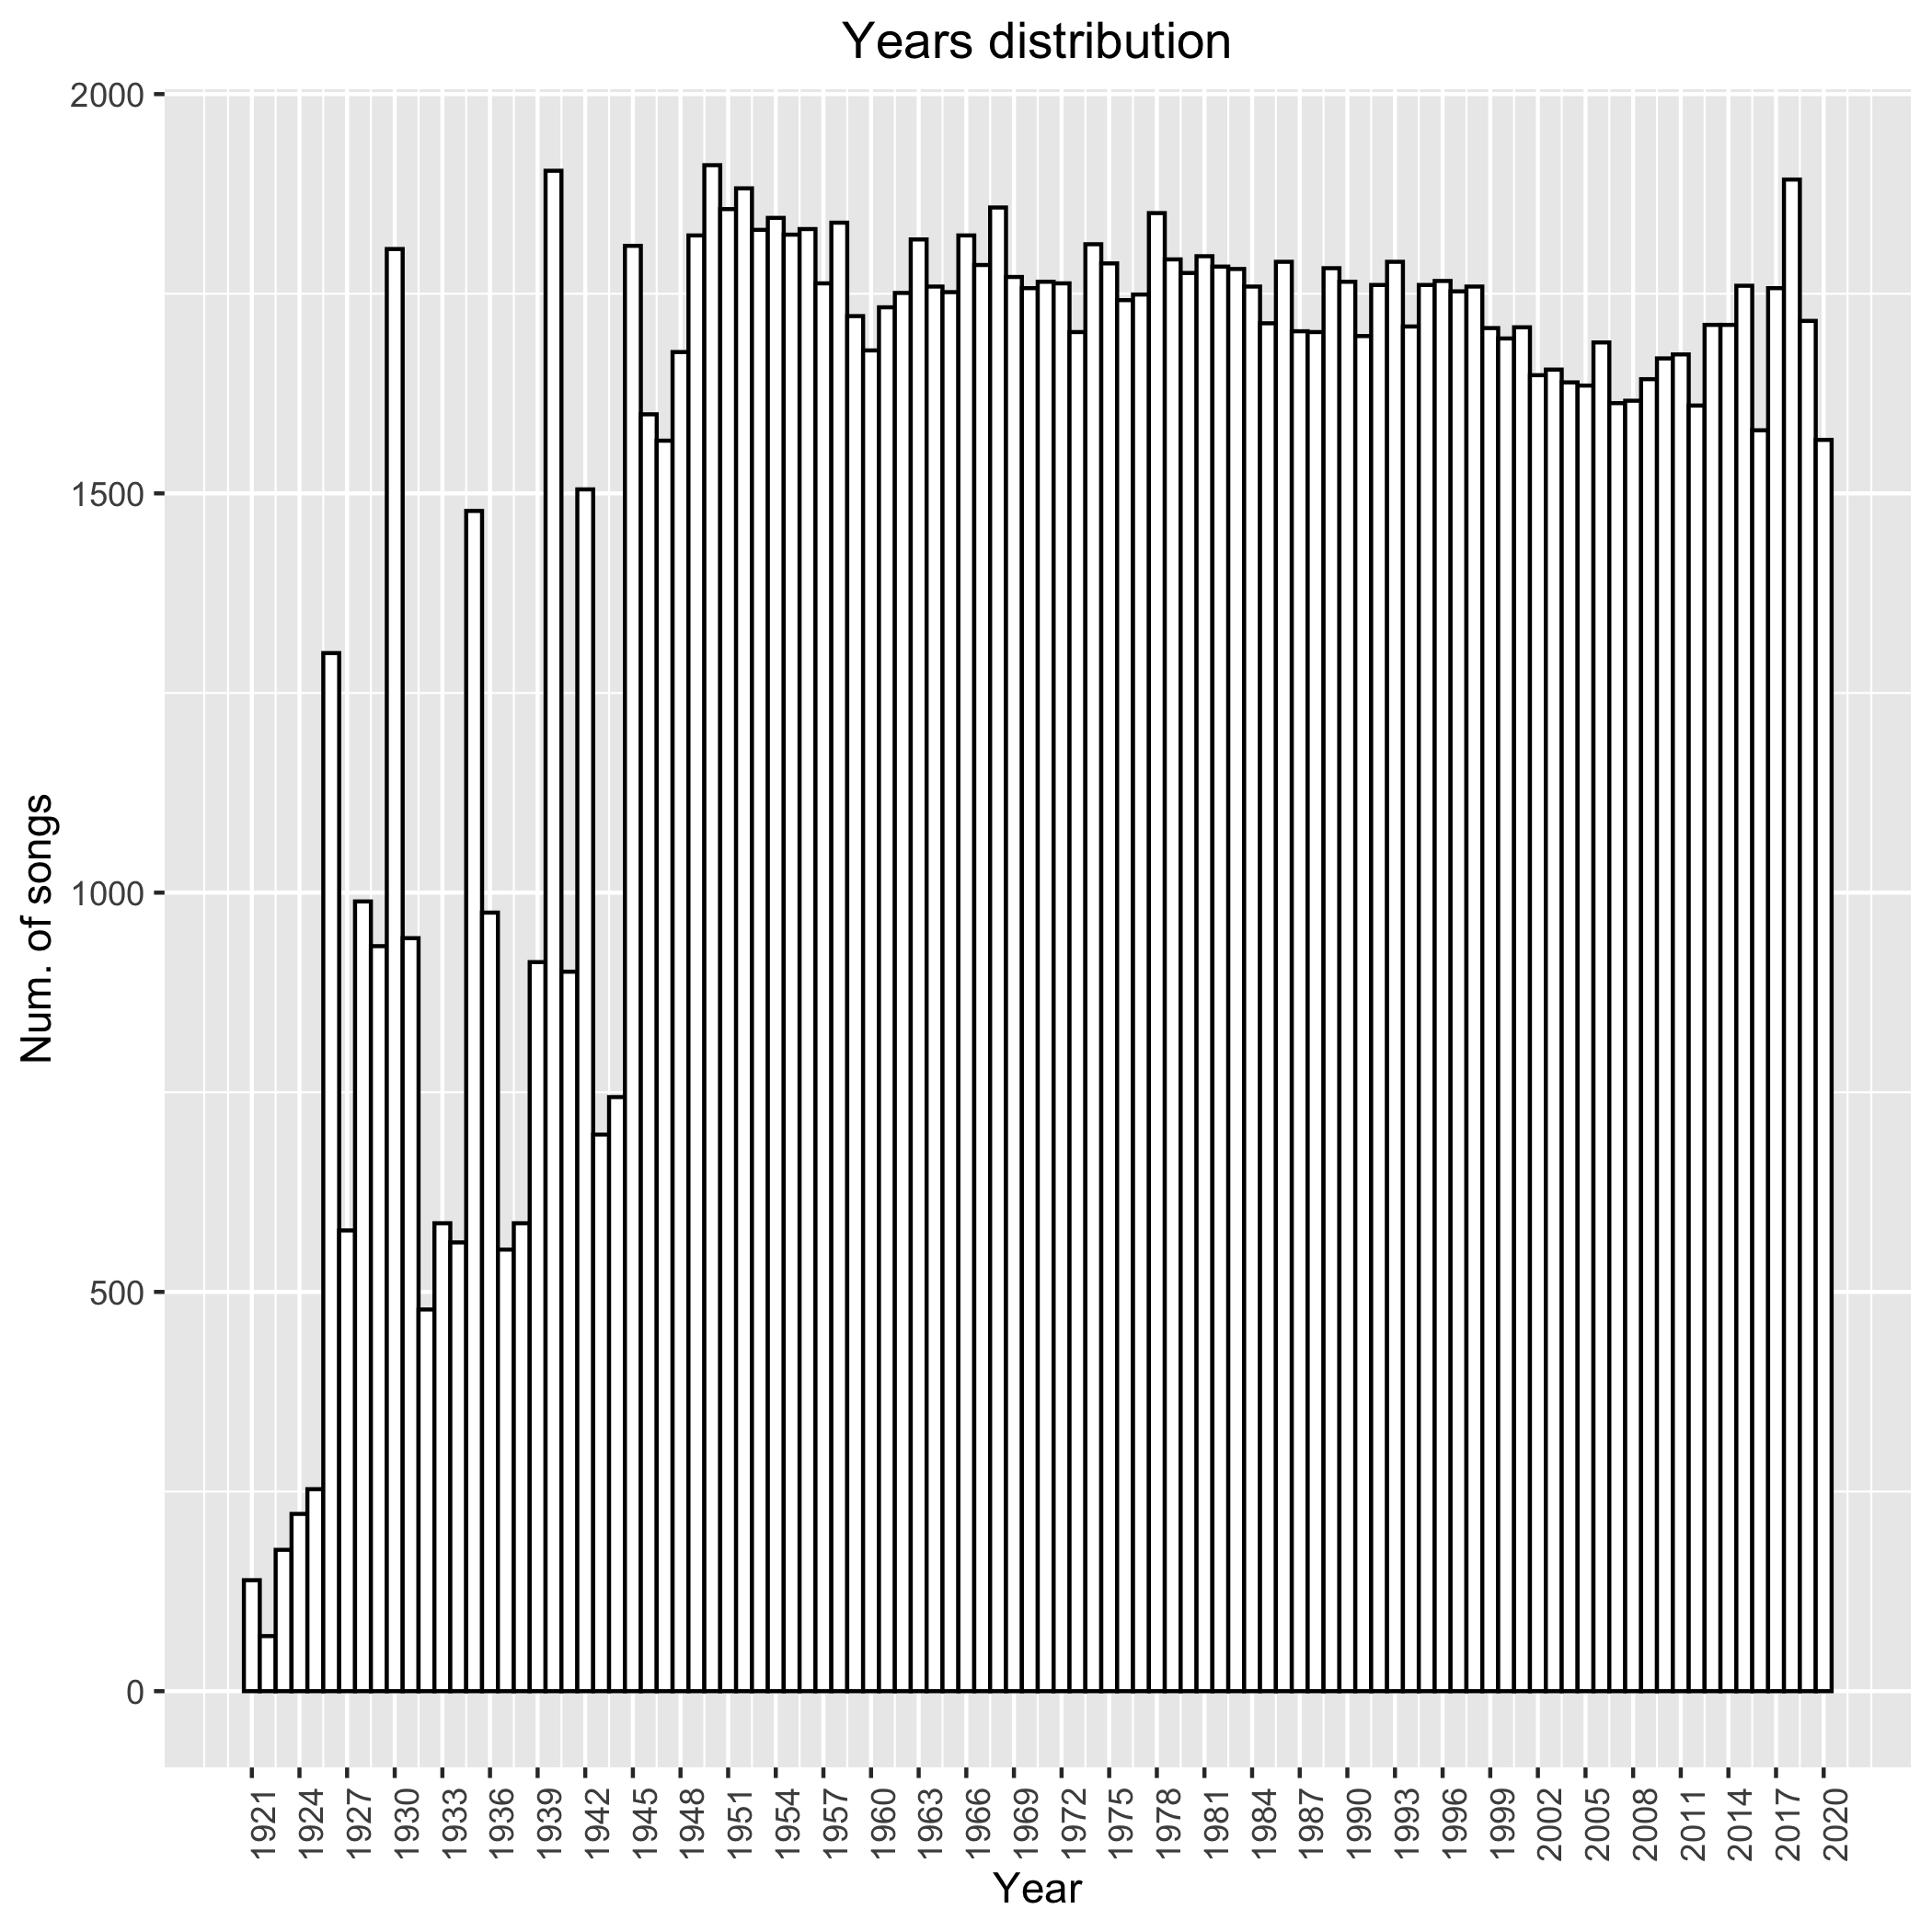
\includegraphics[width=13cm]{../images/years_distribution.png}
	\caption{Distribuzione anno delle canzoni considerando tutto il dataset.}
	\label{fig:year_distribution_all}
\end{figure}

Le diverse certificazioni come "Disco d'oro" e "Disco di platino"
vengono rilasciate considerando il numero di streaming oltre che alle
vendite solo da pochi anni. Inoltre con il passare del tempo i trend
musicali cambiano, un fattore determinante per fare diventare una
canzone di successo.

Con questa giustificazione si ritiene che sia meglio considerare solo
i brani musicali dopo un certo anno di uscita. Prendiamo quindi in
considerazione solo le canzoni dopo il 2005.

La distribuzione delle canzoni dal 2005 in poi è rappresentata in
\autoref{fig:year_distribution_all}. Viene di seguito mostrato il
boxplot delle canzoni dopo quella data distinguendo tra classe
positiva e negativa, così da vedere se esistono differenze.

 \begin{figure}[H]
 	\centering
 	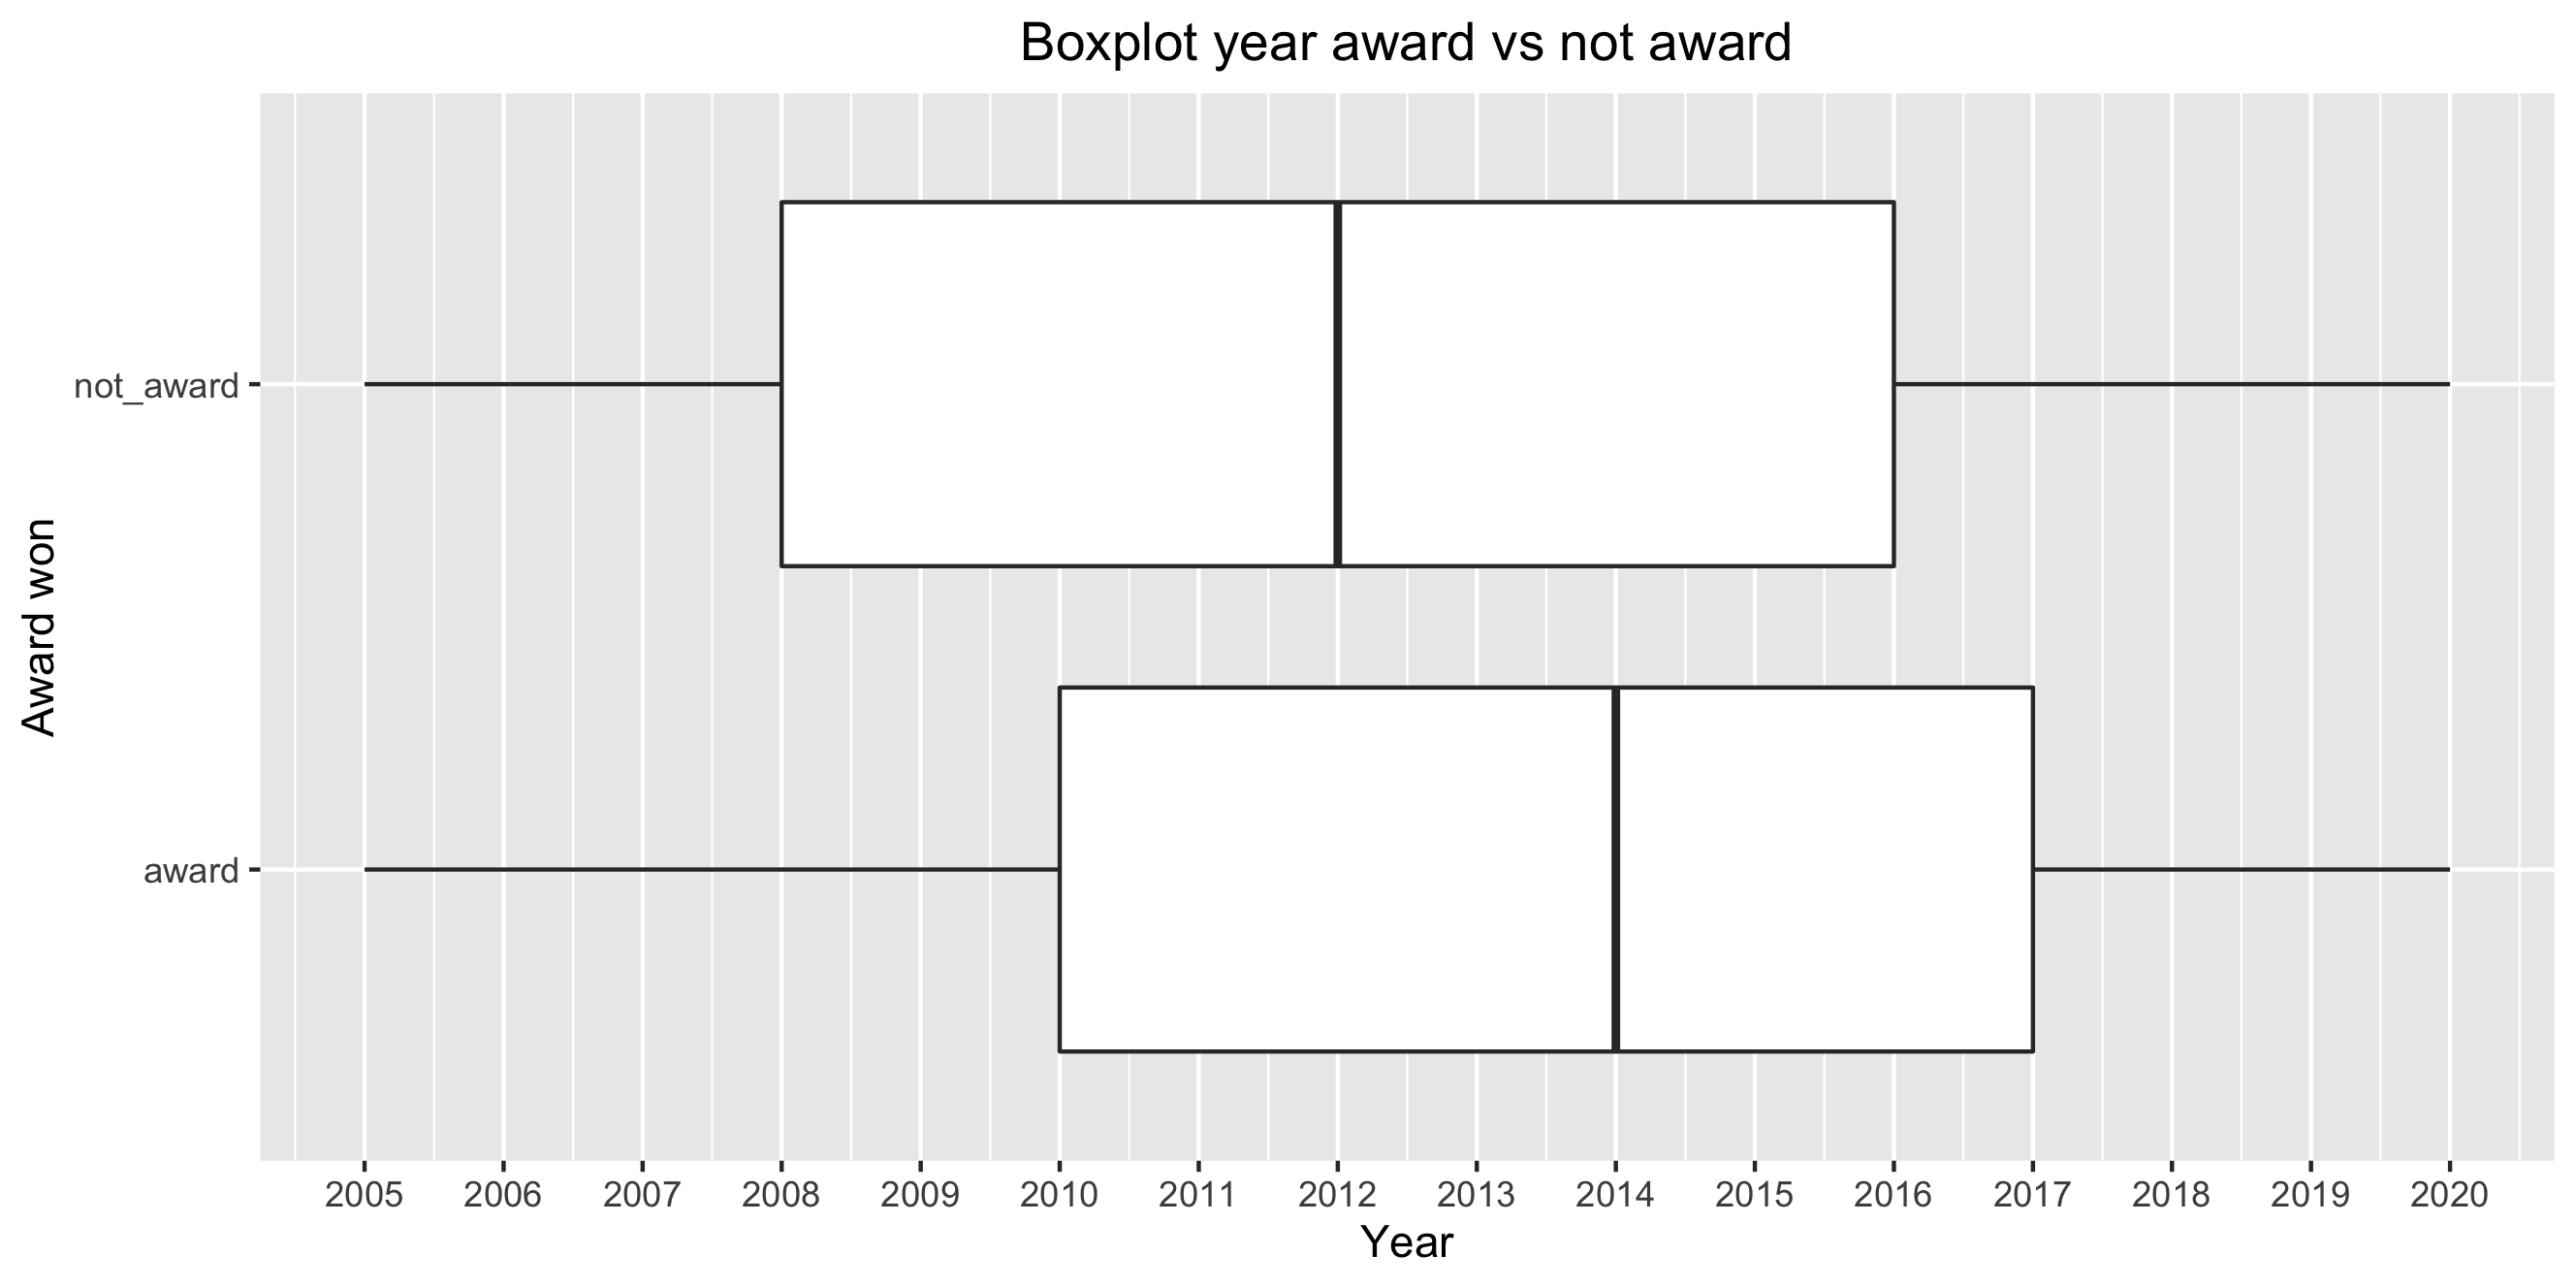
\includegraphics[width=13cm]{../images/year_award_comparison.png}
 	\caption{Boxplot anno di rilascio, distinguendo tra le classi.}
 	\label{fig:year_boxplot_award}
 \end{figure}
 
\subsubsection{Popolarità}
\label{sec:popularity}
Un altro aspetto che viene analizzato a parte, riguardo il quale è
necessario fare ulteriori assunzioni, è il campo popolarità.

Il dataset fornito da Spotify contiene un campo "popularity". Tuttavia
come spiegato nella \autoref{sec:successo}, questo campo non viene
utilizzato per etichettare una canzone come di successo, si utilizza
invece l'informazione delle certificazioni vinte da una canzone
(ottenute da wikipedia).

Il campo "popularity" non verrà usato nella fase di training dei
modelli, proprio perchè è un dato che non si conosce a priori nel
momento in cui un singolo esce, ed è chiaramente influente nel
determinare se una canzone vincerà o meno una certificazione e quindi
se viene considerata di successo.

L'informazione sulla popolarità viene calcolata sul numero di
streaming dopo un determinato lasso di temo. Stimare questo valore,
dal momento che non è conosciuto fin da subito, è di fatto un problema
di regressione ed è molto simile al task di classificazione preso in
esame, pertanto il campo viene scartato.

Anche se il campo non viene effettivamente utilizzato, è interessante
analizzare la distribuzione dei valori di popolarità delle canzoni nel
dataset. Inoltre assumiamo che per il problema trattato, si vogliano
classificare delle canzoni che non sono completamente
sconosciute. Sarebbe infatti irrealistico pensare che un singolo
musicale del tutto sconosciuto vinca dal nulla una certificazione,
risultando come brano di successo.  Per questo motivo non si tratta di
una assunzione molto restrittiva.

Si assume di voler utilizzare questi modelli per classificare brani
che iniziano ad essere un minimo conosciuti o hanno almeno il
potenziale di diventare popolari. Si noti come un brano di poco
popolare non implica assolutamente che questo vinca un disco d'oro o
di platino.

Di seguito viene analizzata da distribuzione della popolarità delle
canzoni nel dataset.


\begin{figure}[H]
	\centering
	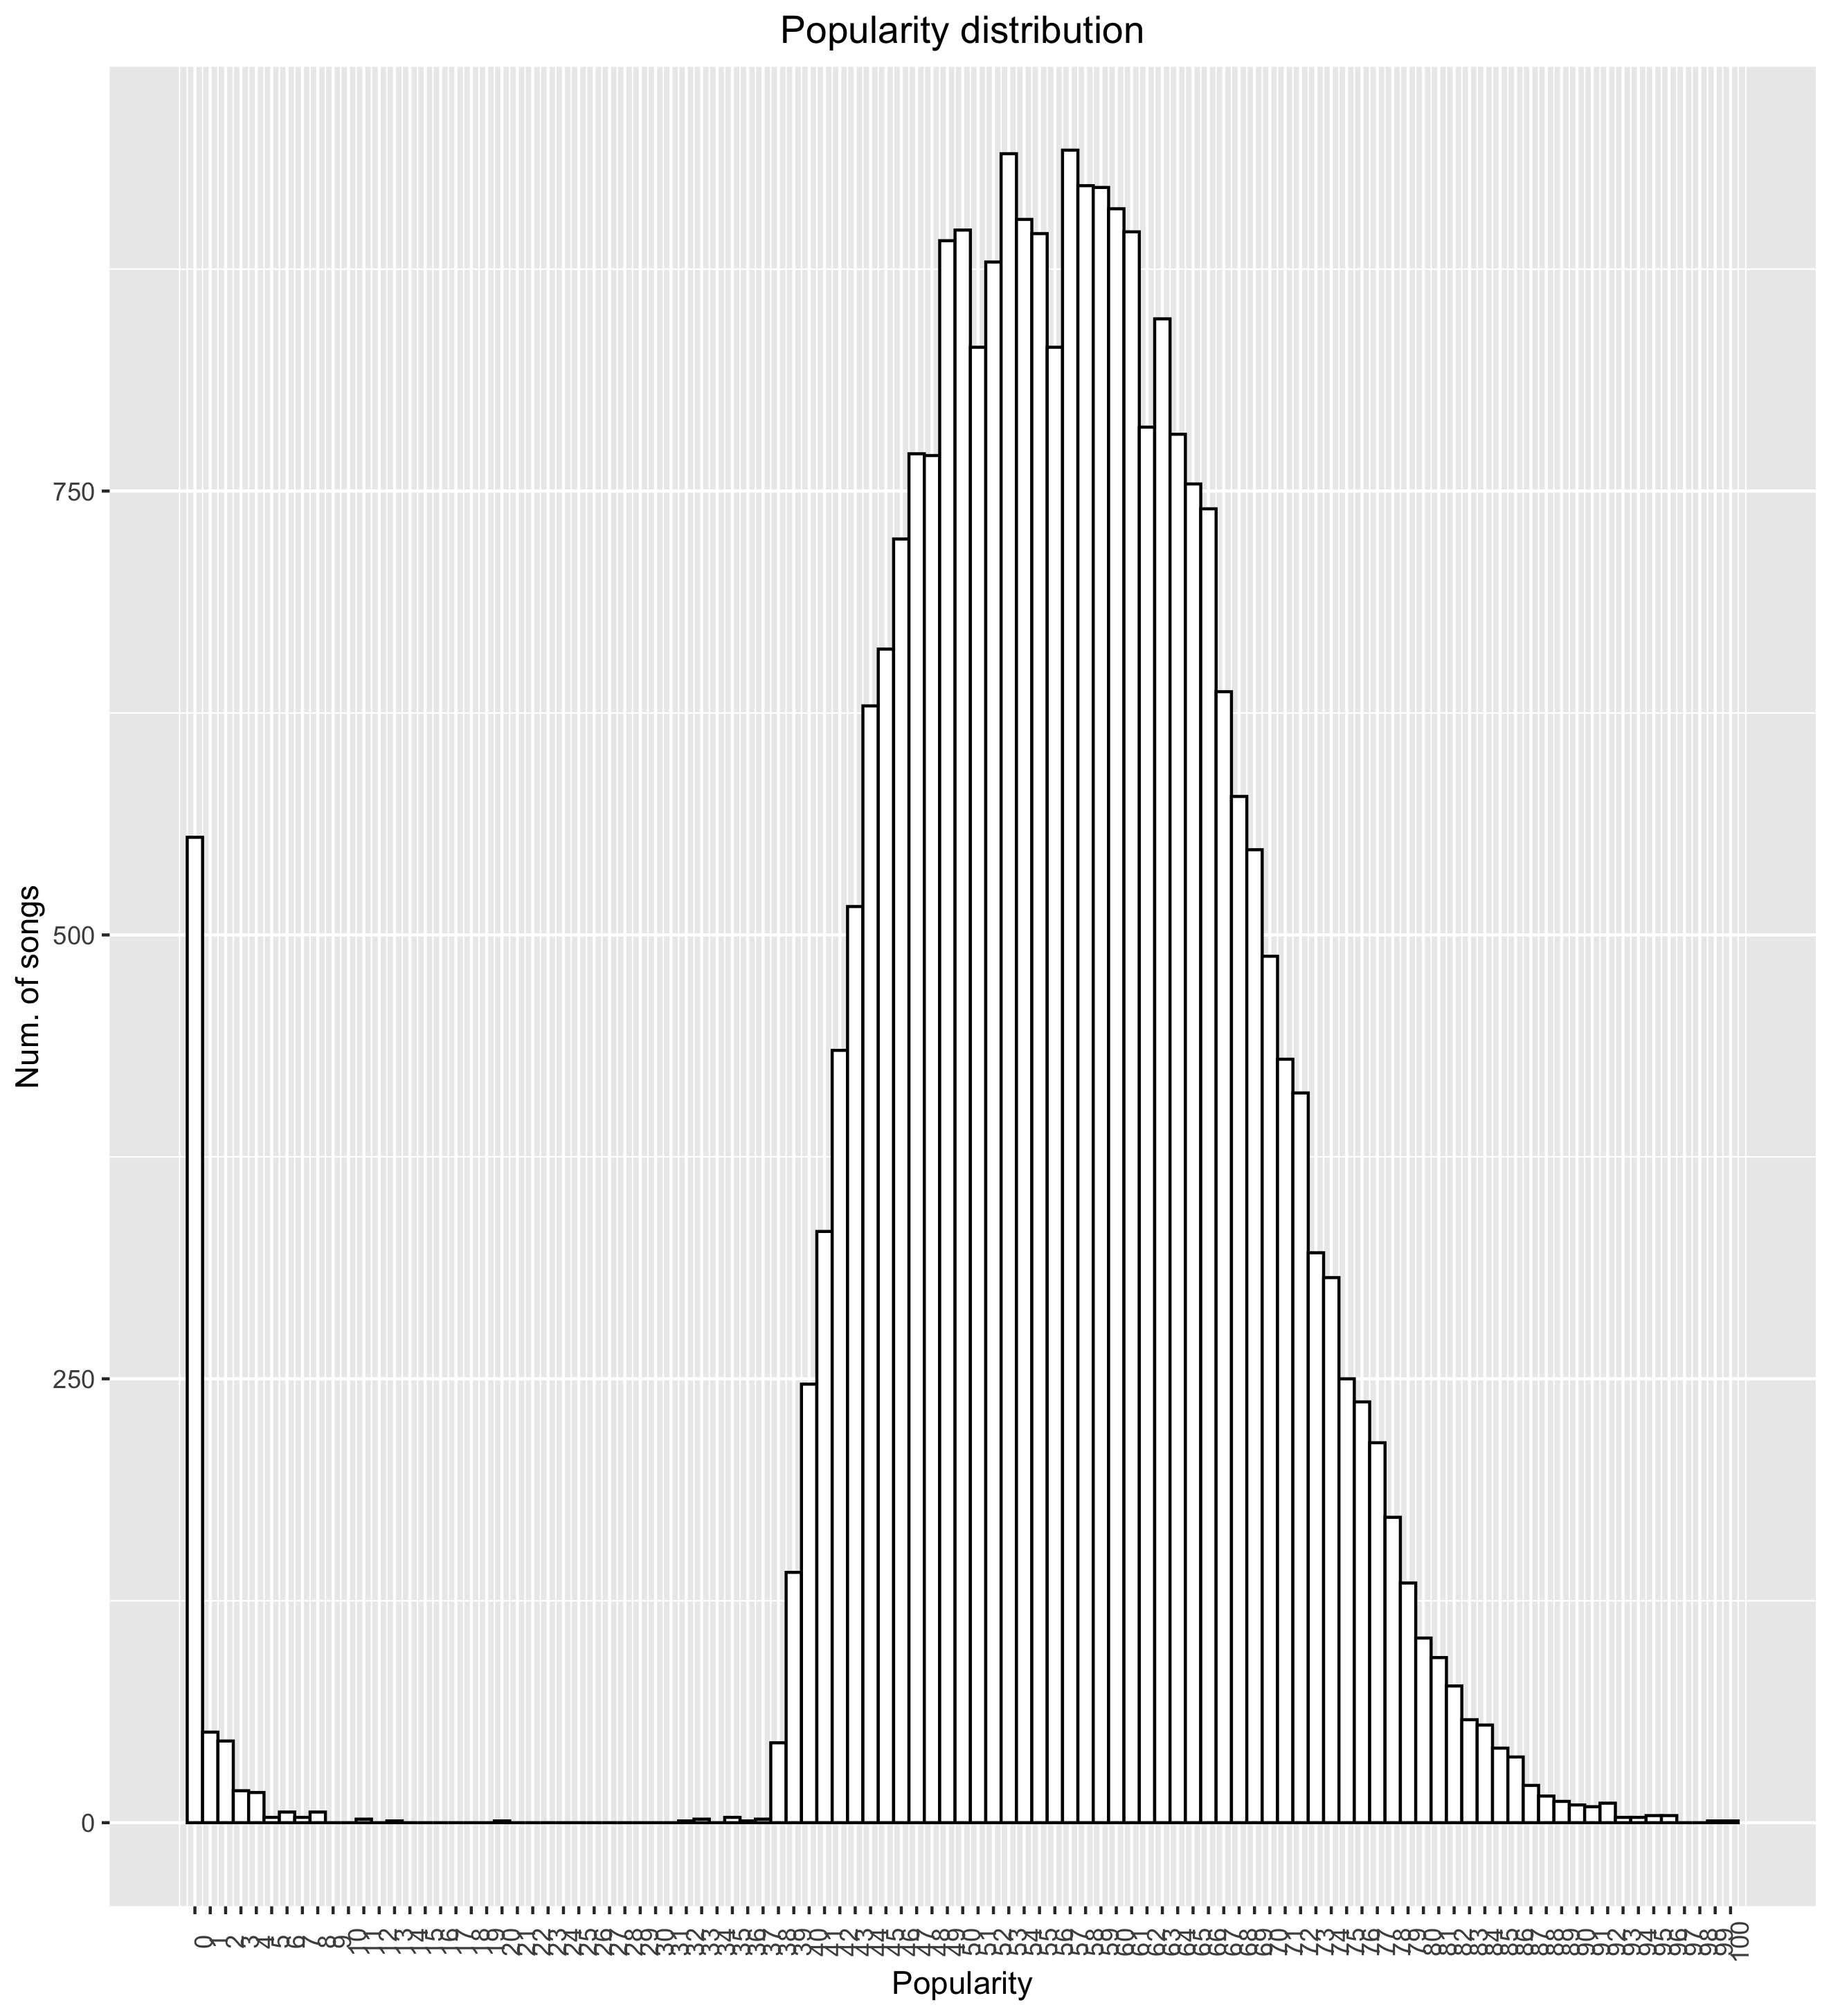
\includegraphics[width=13cm]{../images/popularity_distribution.png}
	\caption{Distribuzione popolarità brani musicali.}
\end{figure}

\begin{figure}[H]
\centering
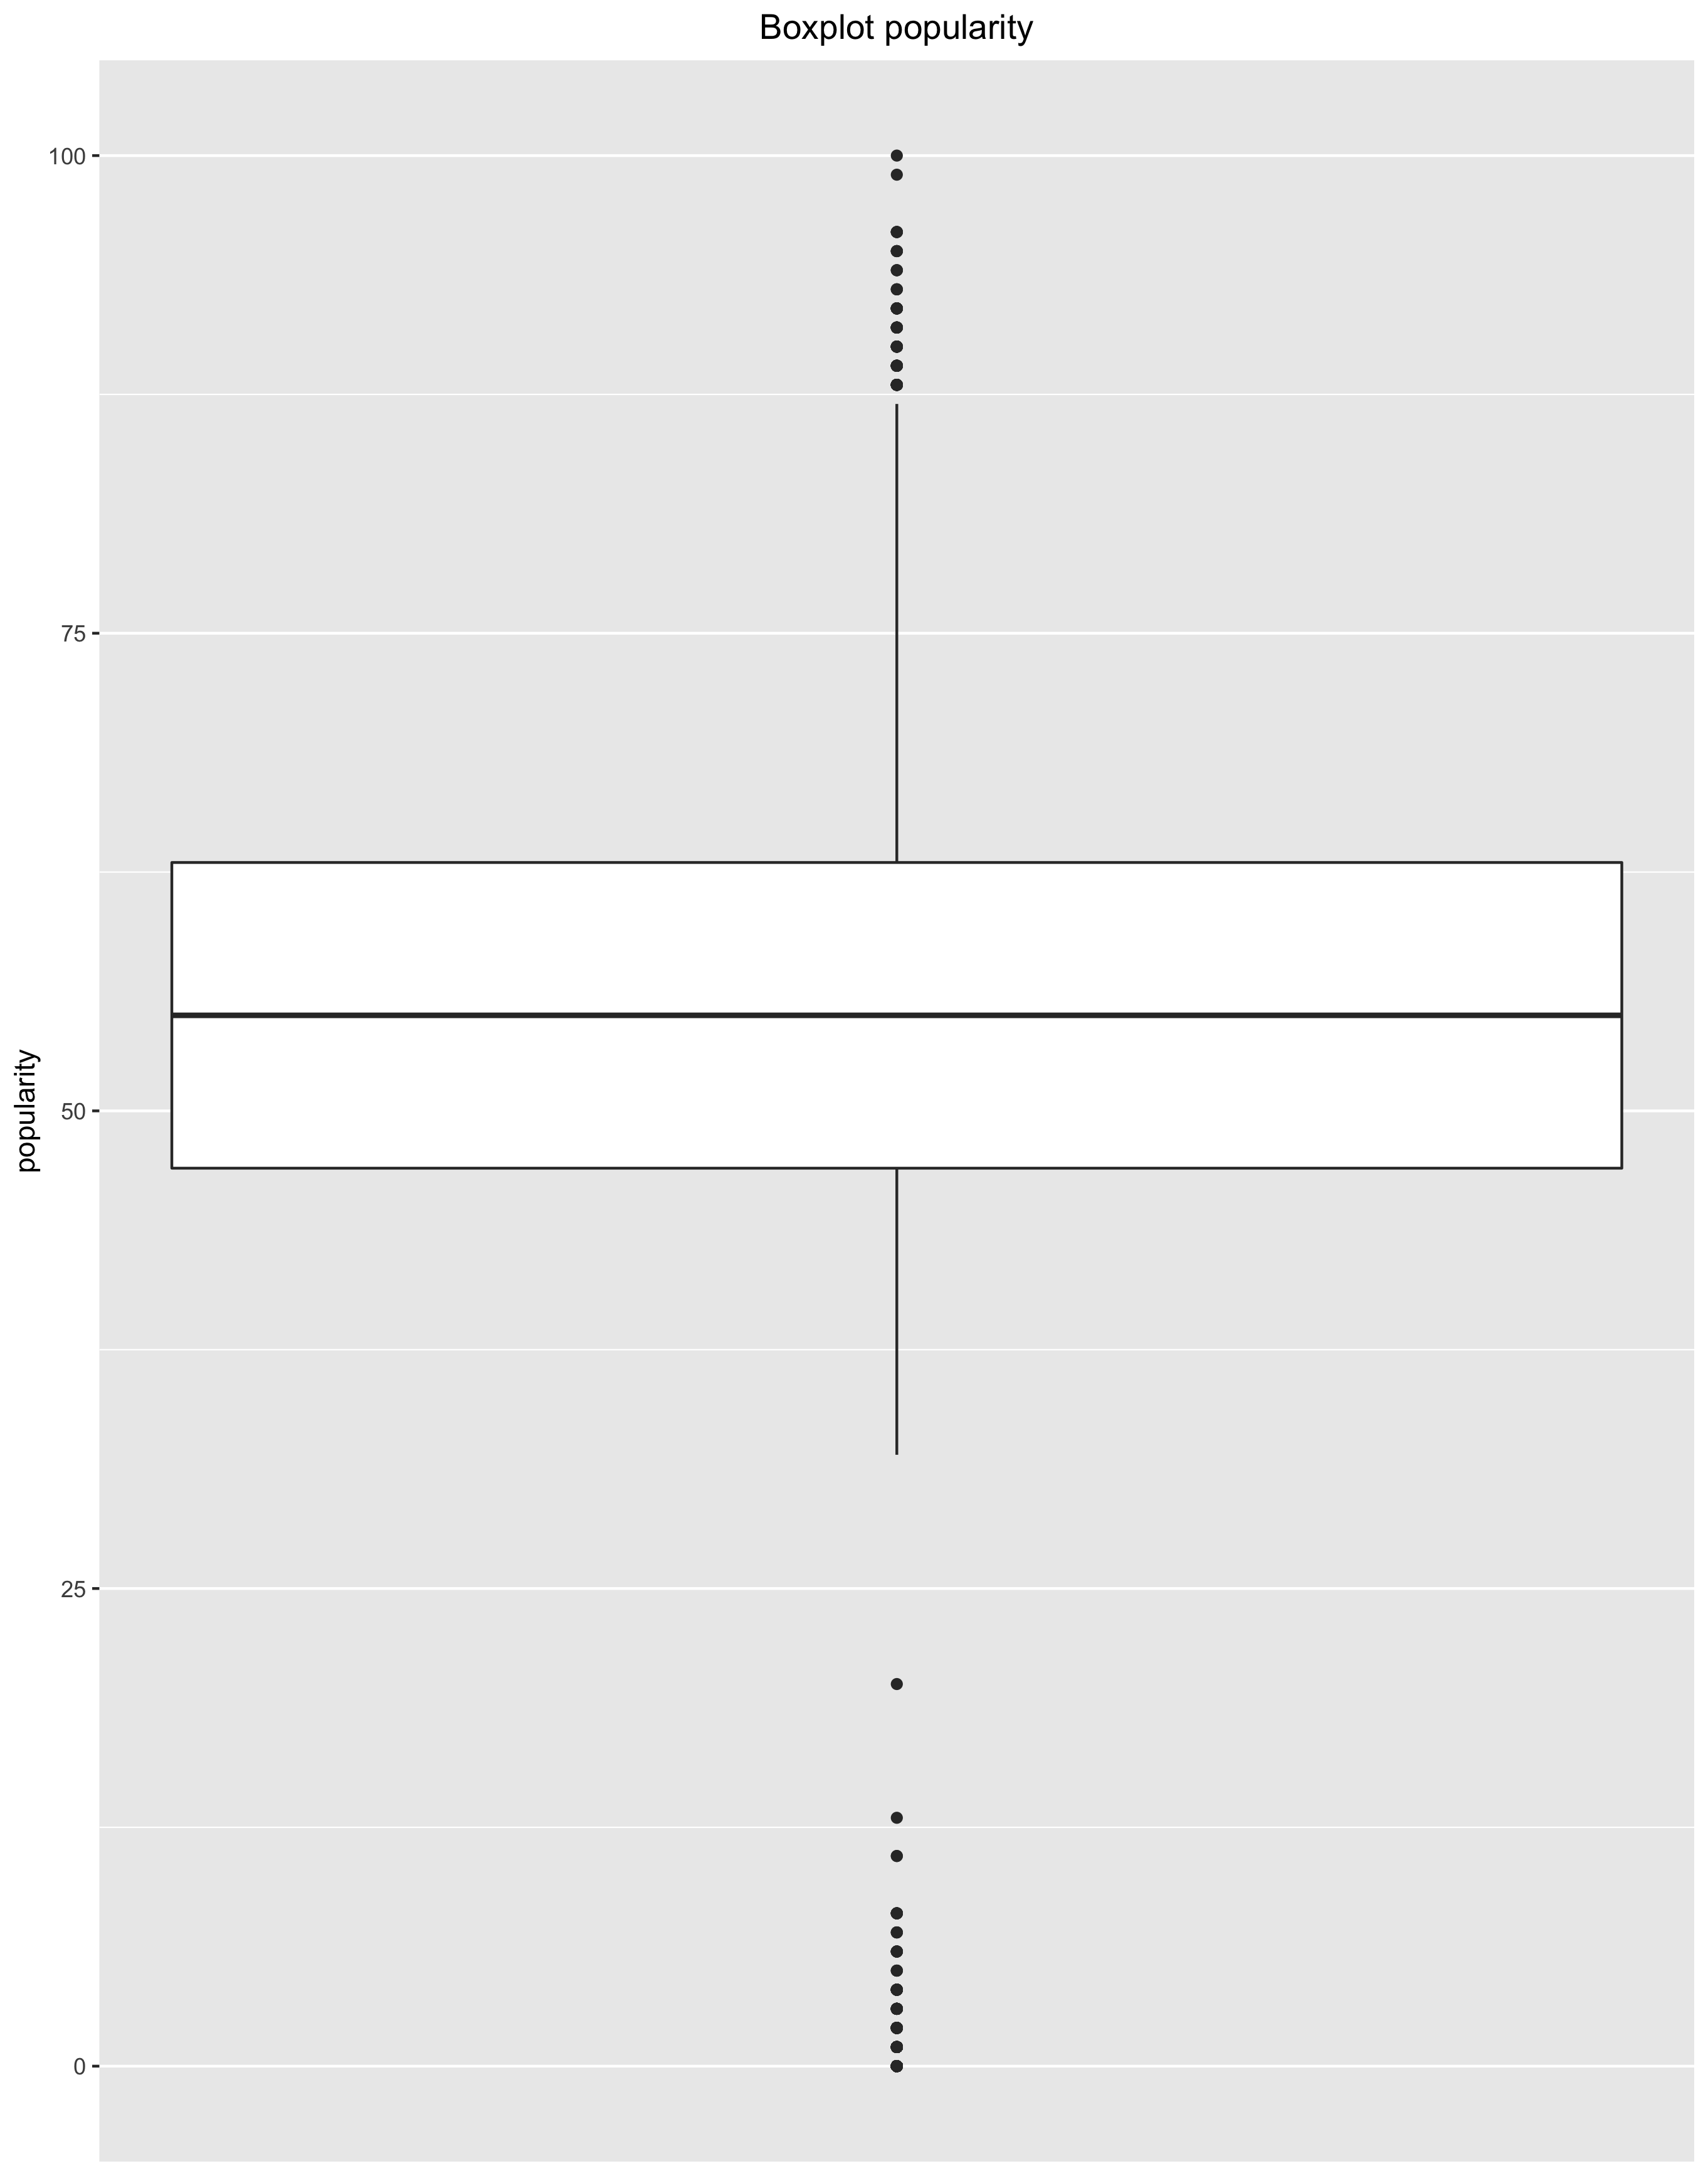
\includegraphics[width=14cm]{../images/popularity_boxplot.png}
\caption{Boxplot popolarità dei brani musicali.}
\end{figure}

Analizzando la distribuzione dei valori della popolarità si
considerano il primo, secondo e terzo quartile, rispettivamente:
$q_{1/4} = 49; \; q_{2/4}= 57; \; q_{3/4} = 65$. Inoltre i valori di
media e deviazione standard sono: $\mu = 57.83; \; \sigma = 10.12$.

Analizzando la distribuzione dei valori della popolarità viene scelto
25 come threshold, valore 3 volte più estremo della deviazione
standard. Si considerano quindi solo i singoli con il valore
"popularity" magggiore del threshold. In questo modo il dataset
rispecchia l'assunzione sopra spiegata riguardo la popolarità minima,
tuttavia si scartano solo i valori davvero estremi per non rendere
questa assunzione troppo restrittiva.

Dopo queste operazioni di riduzione del numero di istanze del dataset
in base alle soglie, il numero di istanze diventa $26134$.

\subsection{Creazione dataset bilanciato}
Dopo aver ridotto il dataset in base alle diverse soglie si vuole
vedere il numero di istanze appartenente alla classe positiva e
negativa. Per classe positiva si intendono i brani che hanno vinto un
premio e sono quindi di successo, viceversa per la classe negativa.

\begin{figure}[H]
	\centering
	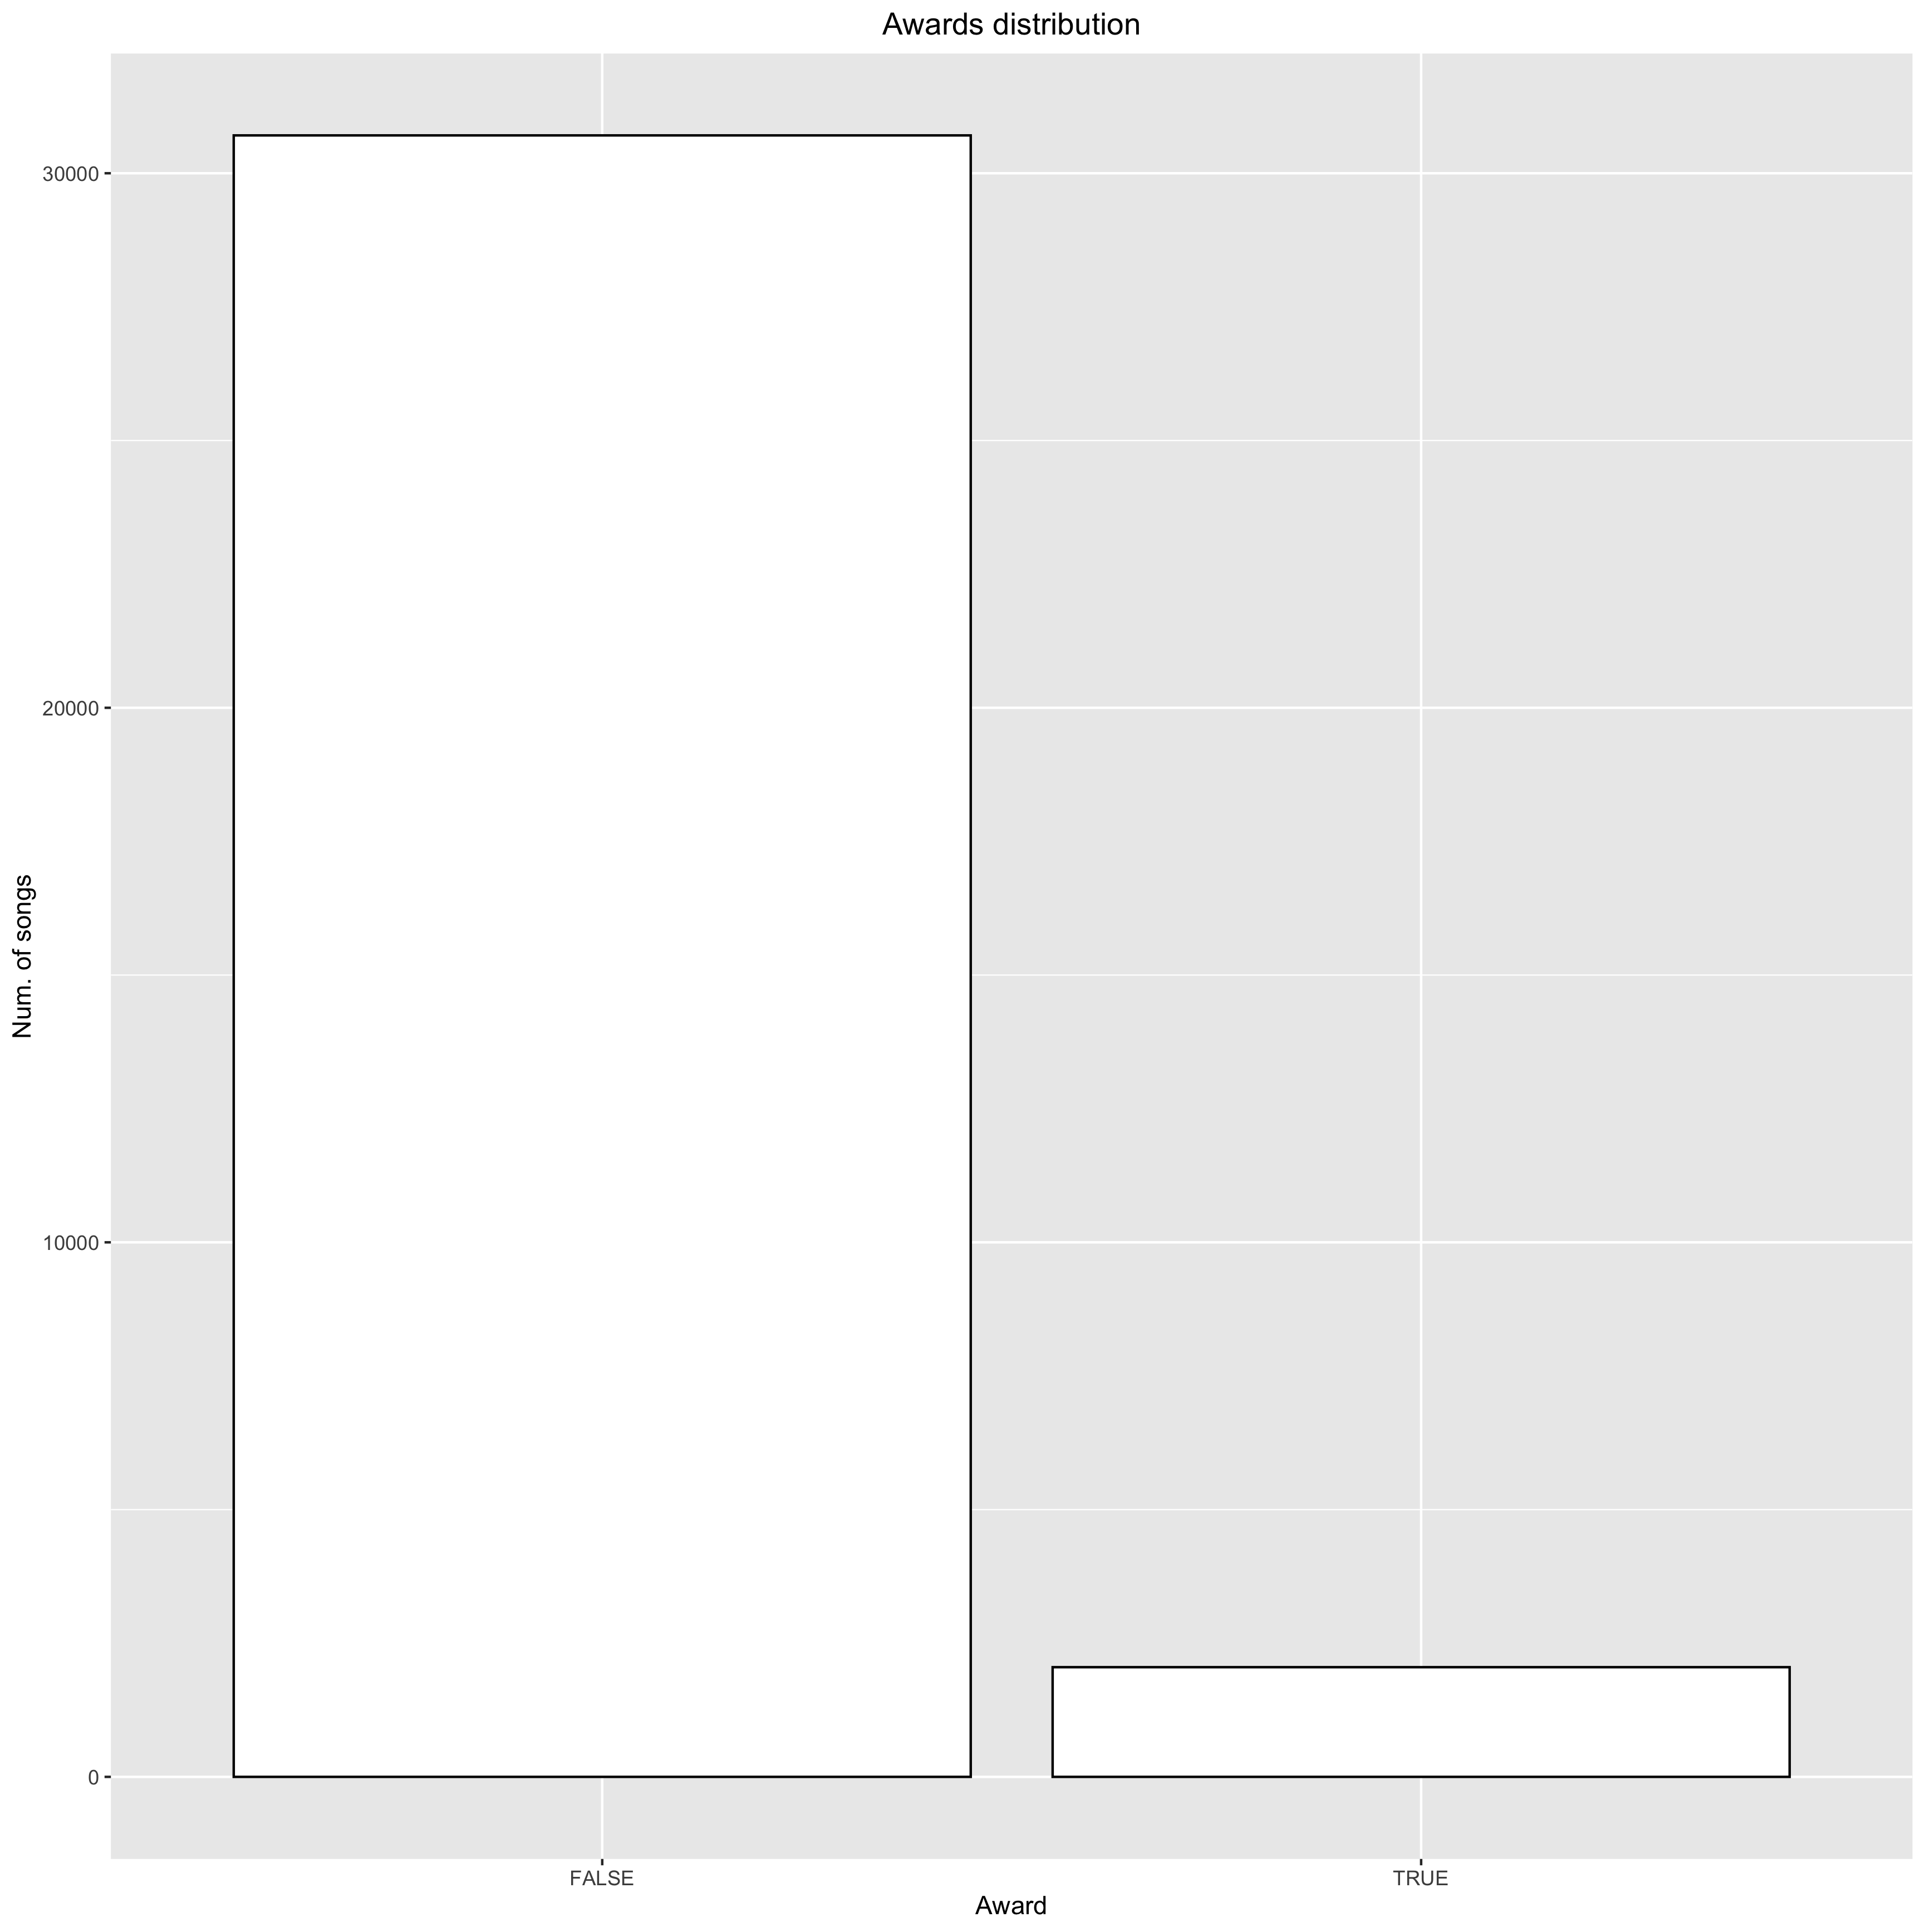
\includegraphics[width=14cm]{../images/awards_distribution.png}
	\caption{Istanze positive e negative.}
	\label{fig:award_distribution}
\end{figure}

\subsubsection{Undersampling}
Dalla \autoref{fig:award_distribution} emerge che il dataset è
sbilanciato, il rapporto tra classe negativa e positiva è circa
$14:1$. Dal momento che questo può creare problemi in fasi di
training, si sceglie di costruire un dataset bilanciato a partire da
tutte le istanze. Come strategia per la costruzione di questo nuovo
dataset vengono scelte casualmente un numero di istanze negative pari
al numero di istanze positive.

\subsection{Preprocessing}
Per quanto riguarda le variabili numeriche queste vengono
standardizzare, ovvero per ogni covariata si trasformano gli individui
in modo da ottenere dei valori tali che $\mu = 0;\; \sigma =
1$. Questa è sicuramente una best practice ma è cruciale per quanto
riguarda la PCA, tecnica che viene utilizzata e spiegata nella sezione
\autoref{sec:pca}.

Inoltre nella fase di preprocessing tutti gli artisti vengono
trasformati in lowercase. Questo è necessario nel momento in cui si
vuole tenere traccia degli artisti nelle canzoni con una
rappresentazione one hot encoding (\autoref{sec:one}).

\subsection{Distribuzione dei valori}
\subsubsection{Variabili numeriche}
Di seguito viene mostrata la distribuzione delle covariate,
distinguendo tra singoli che hanno vinto un premio (Classe positiva) e
quelli che non hanno vinto un premio (Classe negativa).

Dal pairplot della \autoref{fig:pairplot} possiamo notare come non
esiste una netta distinzione nei dati tra brani di successo e brani
non di successo. Questo sarà sicuramente un problema in fase di
classificazione e potrebbe potrare a basse performance dei
modelli. Riteniamo quindi che sia necessario considerare altre
features per ben distinguere brani musicali di successo da quelli non
di successo.

Il campo "popularity" ben distingue le due classi, tuttavia come già
discusso in \autoref{sec:popularity}, questa covariata non verrà
utilizzata per la creazione dei modelli.

Inoltre esiste correlazione tra alcune covariate, come ad esempio tra
"energy" e "loudness", questo rispecchia intuitivamente l'idea di come
una canzone più energica è anche più rumorosa. La correlazione tra le
variabili viene meglio analizzata in \autoref{sec:correlazione}.


\begin{figure}[H]
	\hspace*{-1.5cm}   
	\centering
	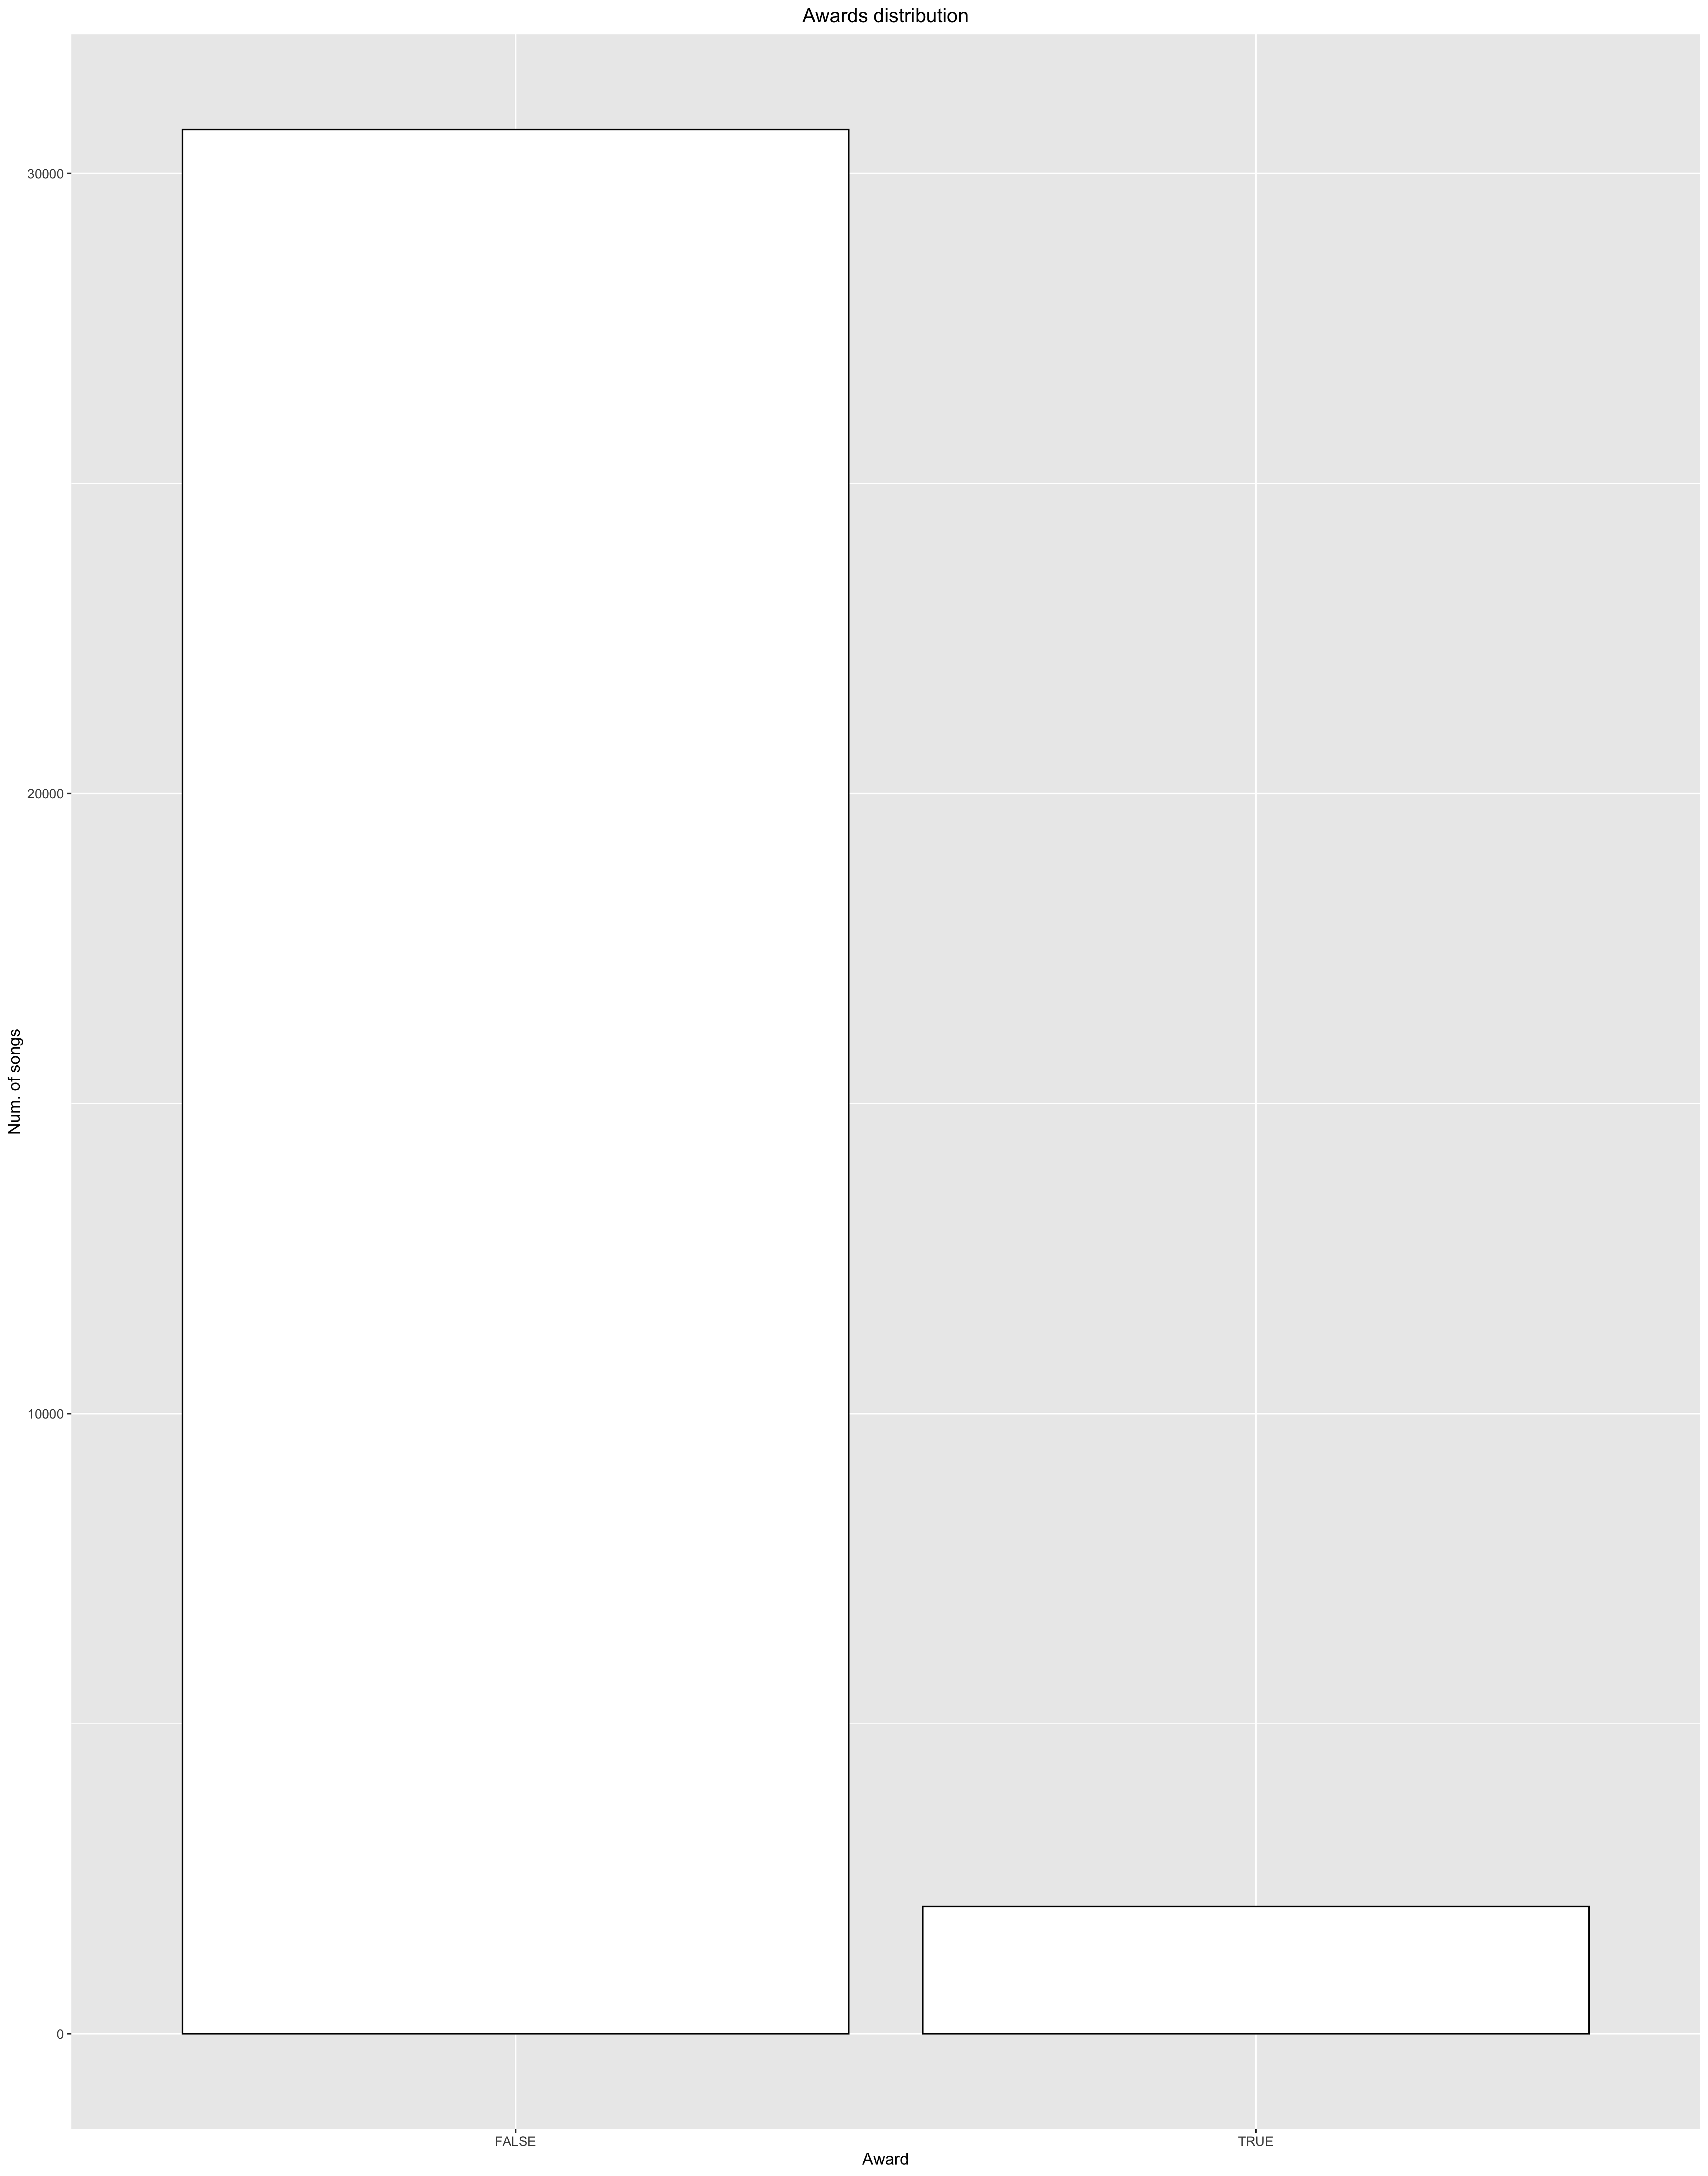
\includegraphics[width=23cm, angle=270]{../images/pairplot.png}
	\caption{Pairplot delle covariate.}
	\label{fig:pairplot}
\end{figure}

\subsubsection{Variabili categoriche}
Di seguito si esplorano le variabili categoriche del dataset,
distinguendo tra classe positiva e negativa.

\begin{figure}[!h]

	\begin{subfigure}[b]{\textwidth}
		\centering
		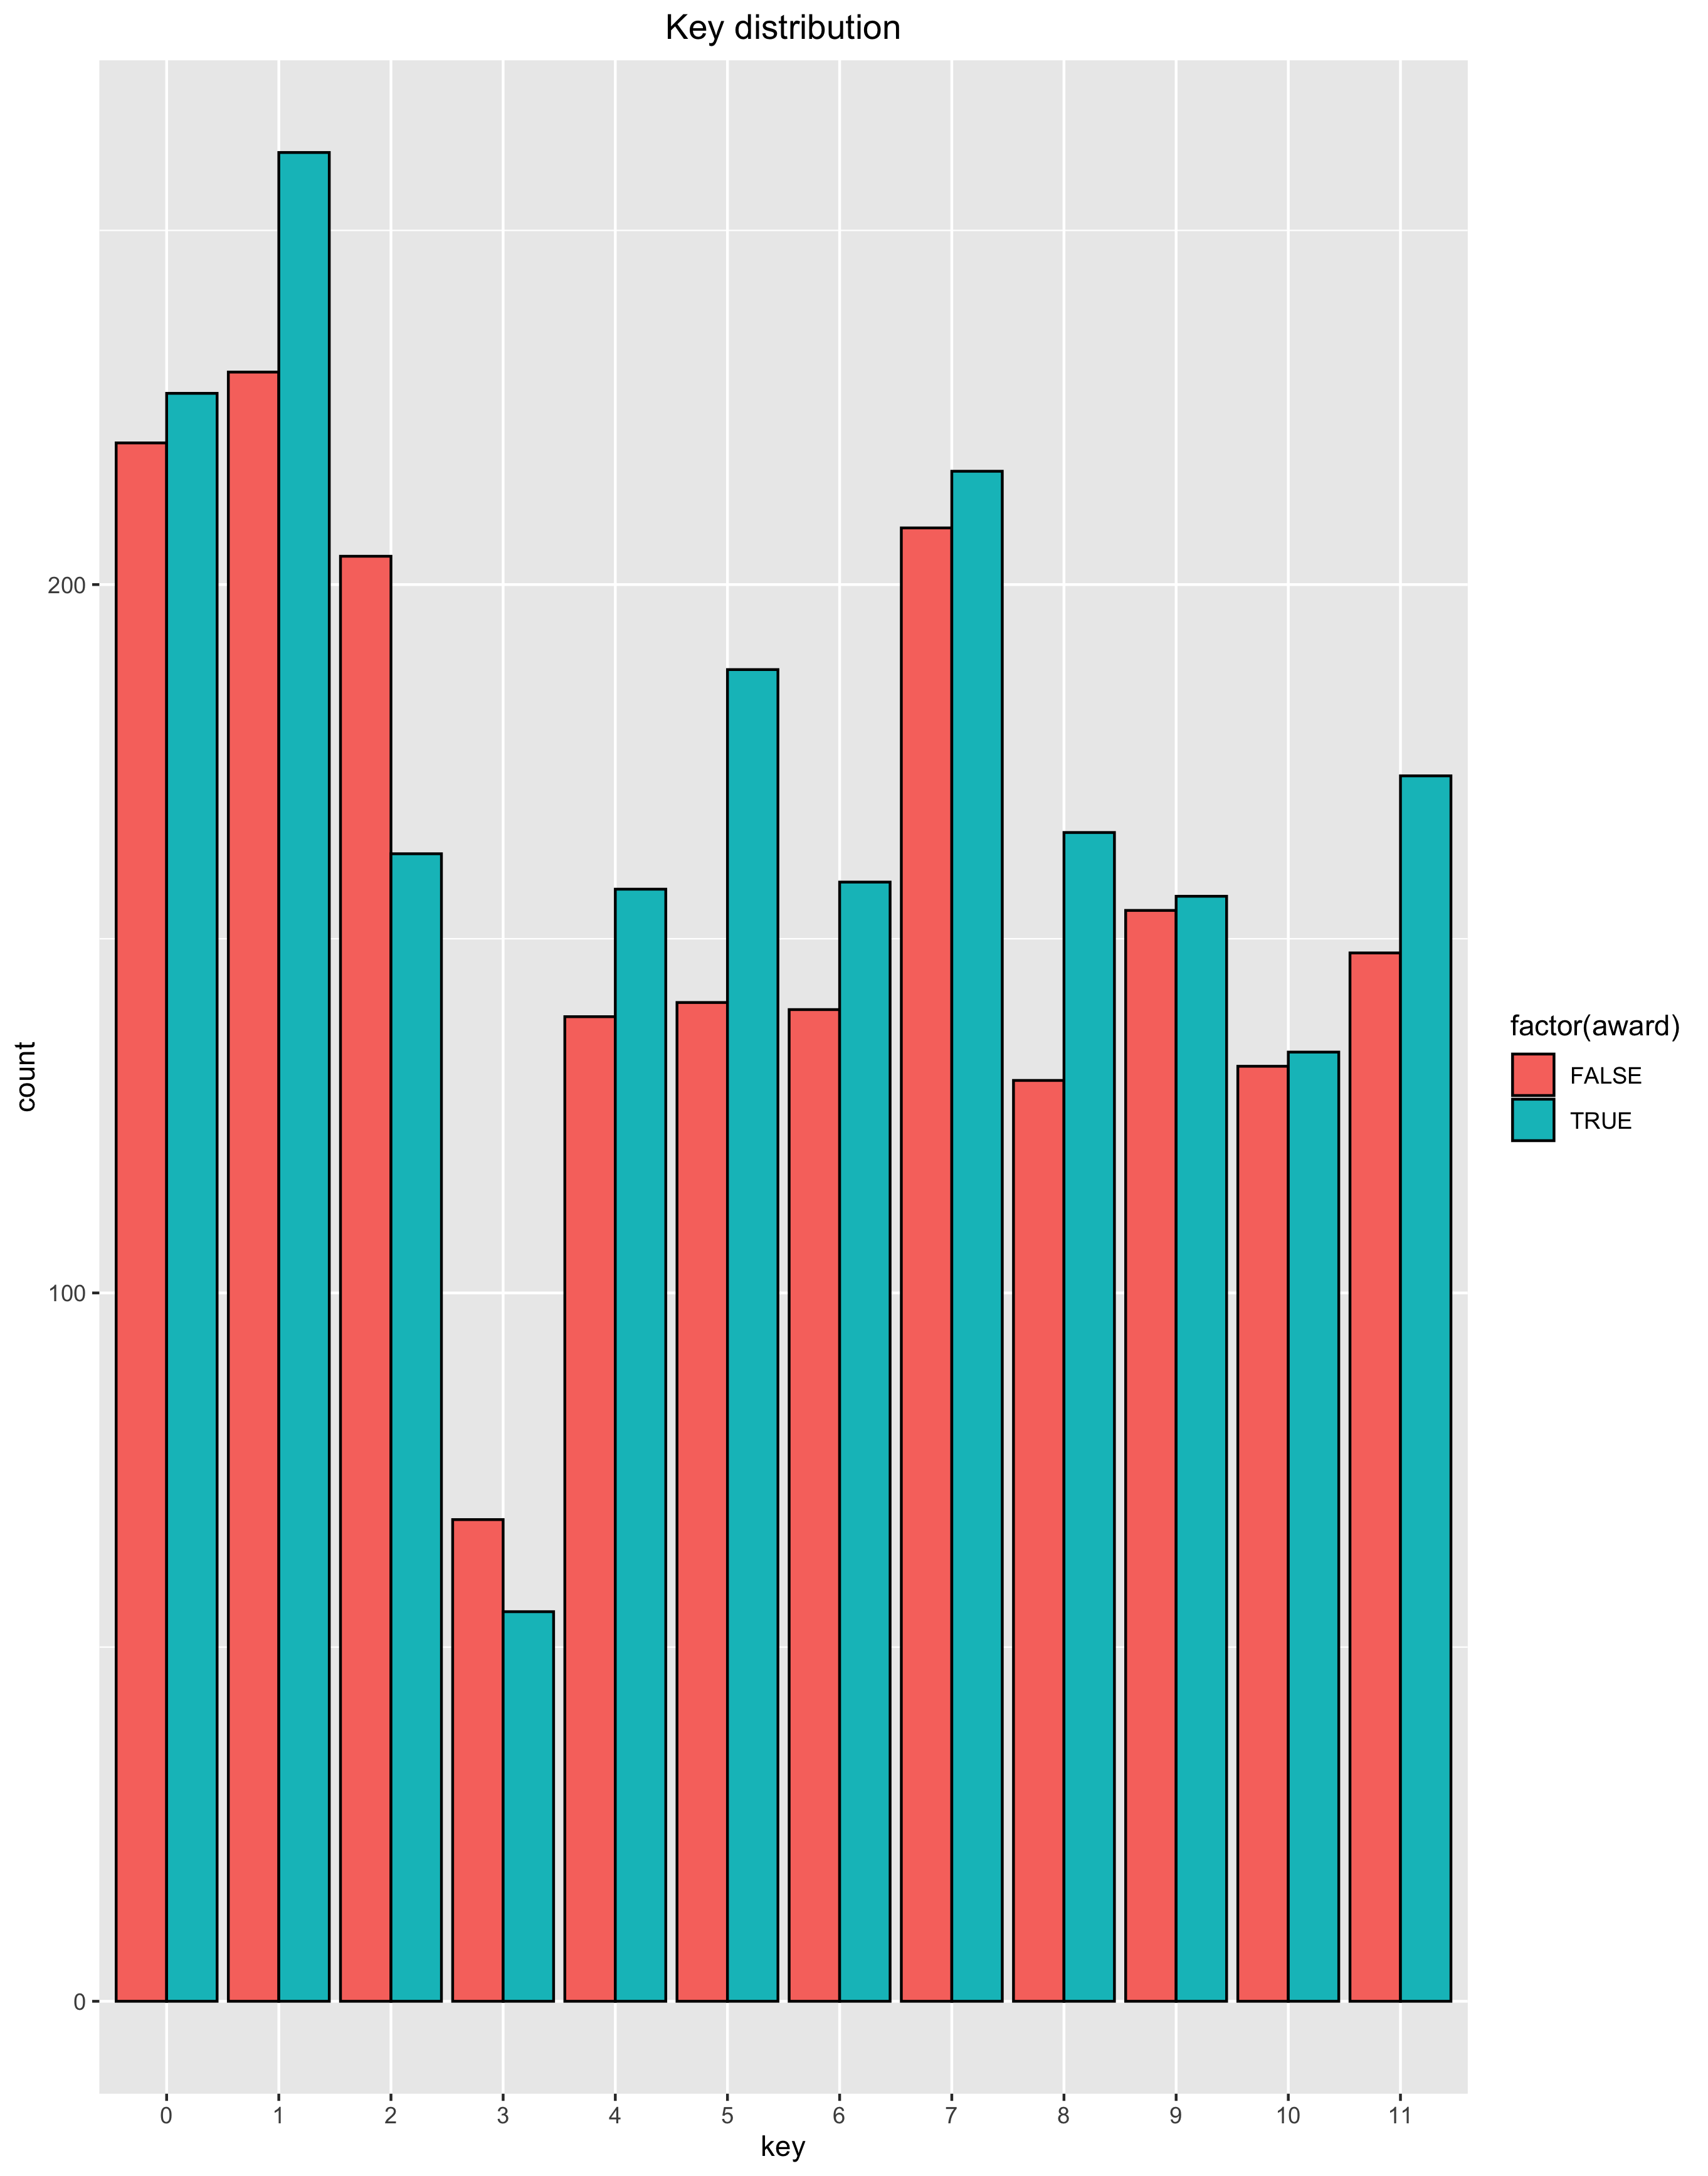
\includegraphics[width=13cm]{../images/key_distribution.png}
		\caption{Variabile key.}
	\end{subfigure}
      
	\begin{subfigure}[b]{0.3\textwidth}
		\centering
		\hspace*{-2cm}   
		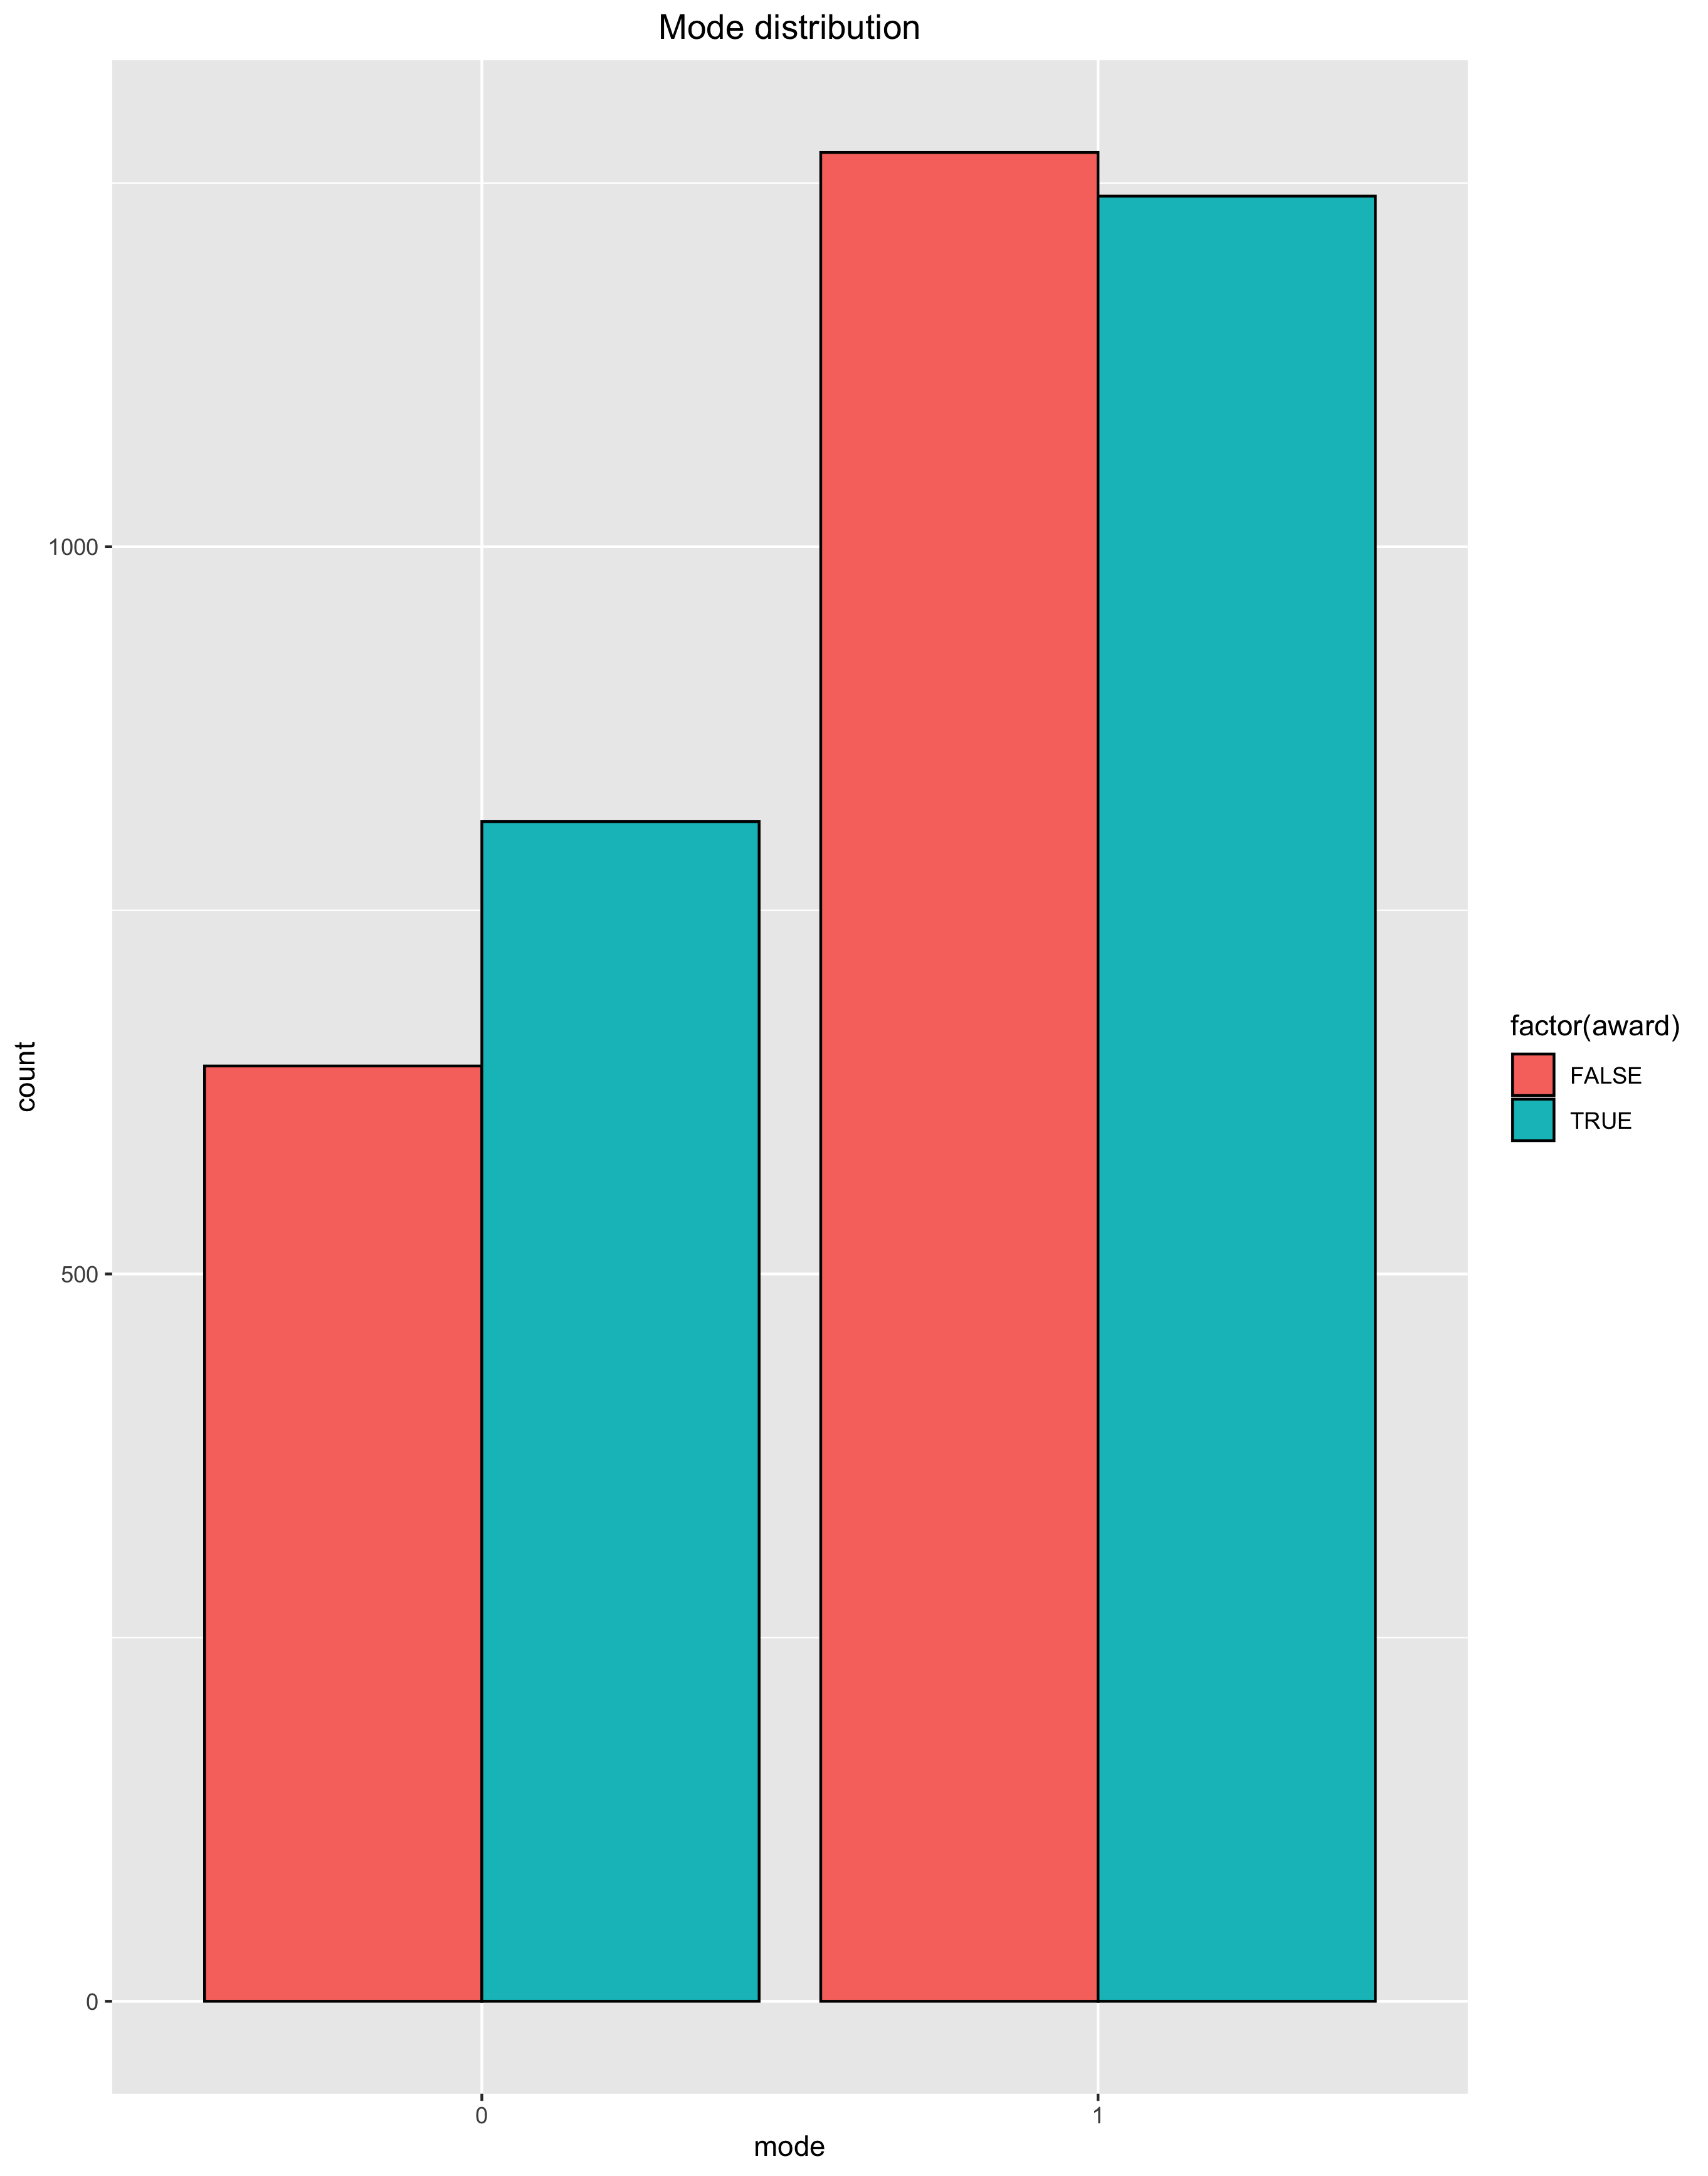
\includegraphics[width=10cm]{../images/mode_distribution.png}
		\caption{Variabile mode.}
	\end{subfigure}
	\hfill
	\begin{subfigure}[b]{0.6\textwidth}
		\centering
		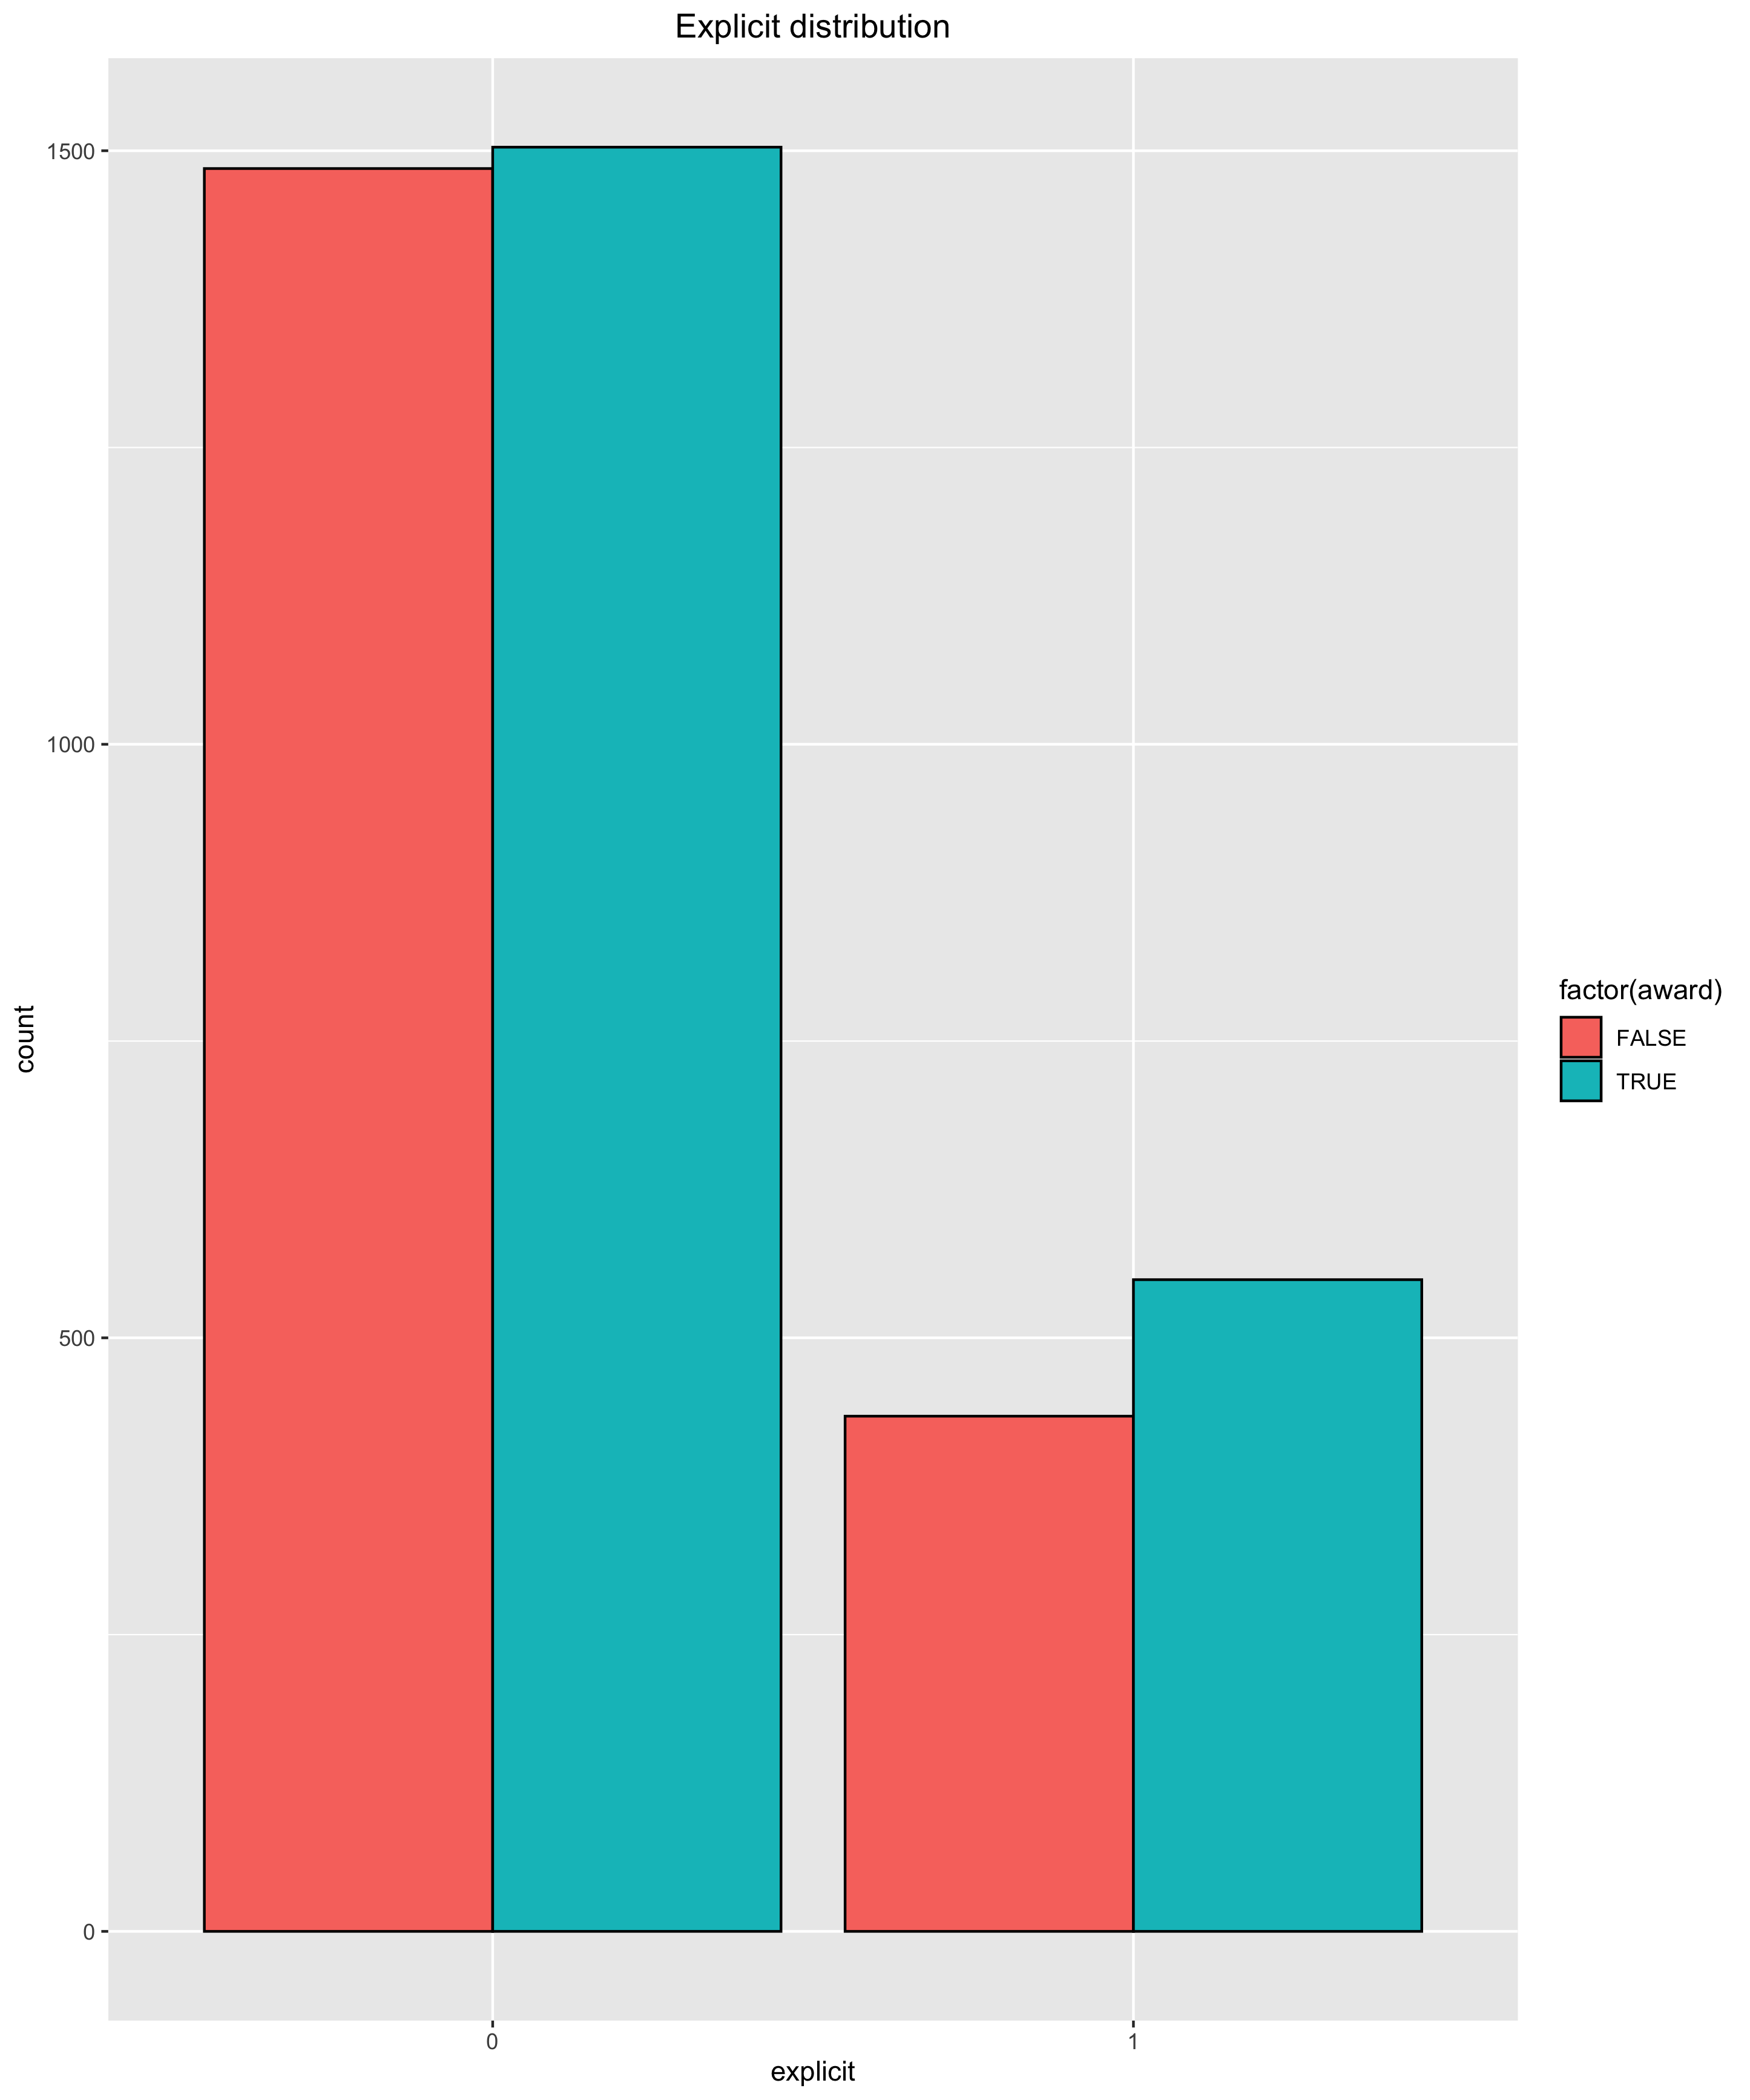
\includegraphics[width=10cm]{../images/explicit_distribution.png}
		\caption{Variabile explicit.}
	\end{subfigure}%
	\caption{Distribuzione delle variabili categoriche.}
\end{figure}

\subsection{Artisti nelle canzoni}
Un'altra caratteristica che si ritiene importante per riconoscere una
canzone come di successo, è quali artisti sono presenti in una
canzone.

\subsubsection{Frequenza artisti}
\label{sec:freq_artisti}
Vine ora considareato il numero di occorrenze di ogni artista tra
tutte le canzoni, si analizza quindi la frequenza delle occorrenze.

\begin{figure}[H]
	\centering
	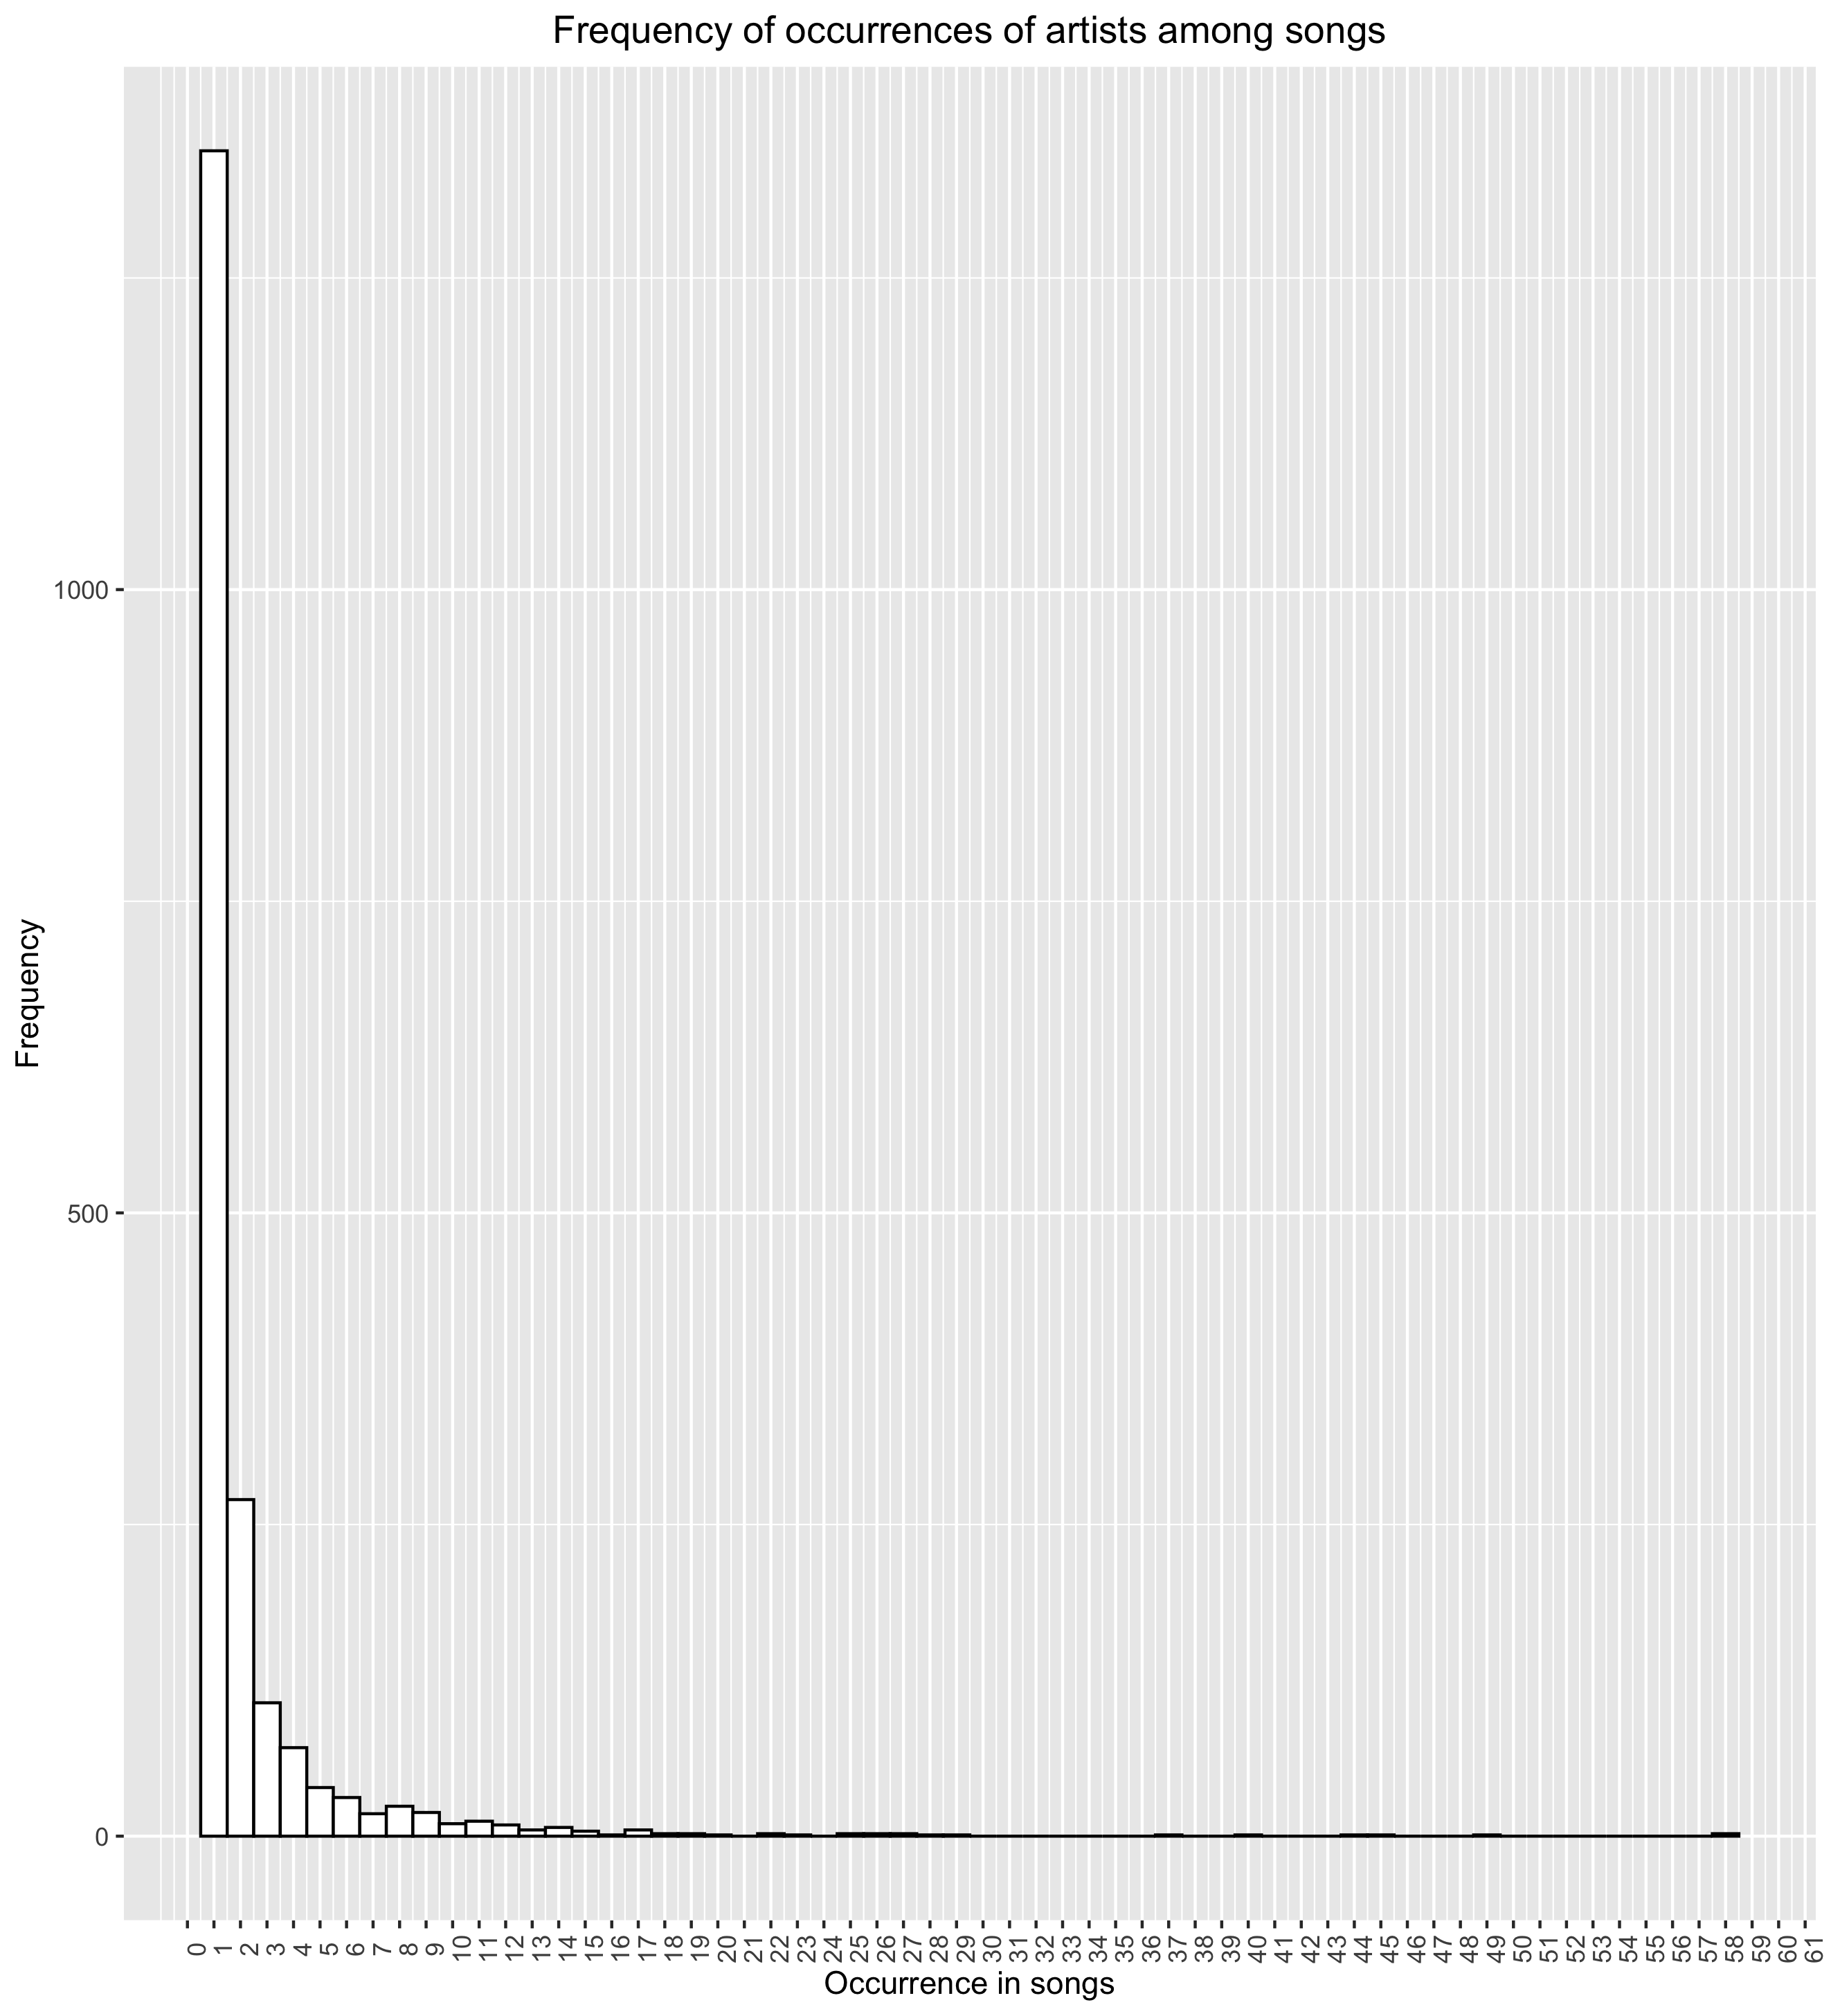
\includegraphics[width=10cm]{../images/artists_occurence.png}
	\caption{Frequenza delle occorenze degli artisti nelle canzoni.}
\end{figure}

Come possiamo notare da questo grafico, la maggior parte degli artisti
hanno fatto solo una canzone. Questo aspetto verrà tenuto in
considerazione per la rappresentazione one hot encoding degli artisti,
come spiegato in \autoref{sec:one}

\subsubsection{Wordcloud}
Si vuole ora analizzare se esiste una differenza tra artisti che hanno
realizzato brani di successo rispetto a quelli non di successo. Viene
prima di tutto mostrato il wordcloud degli artisti tra tutte le
canzoni, senza fare distinzione tra classe positiva e negativa.

\begin{figure}[H]
	\centering
	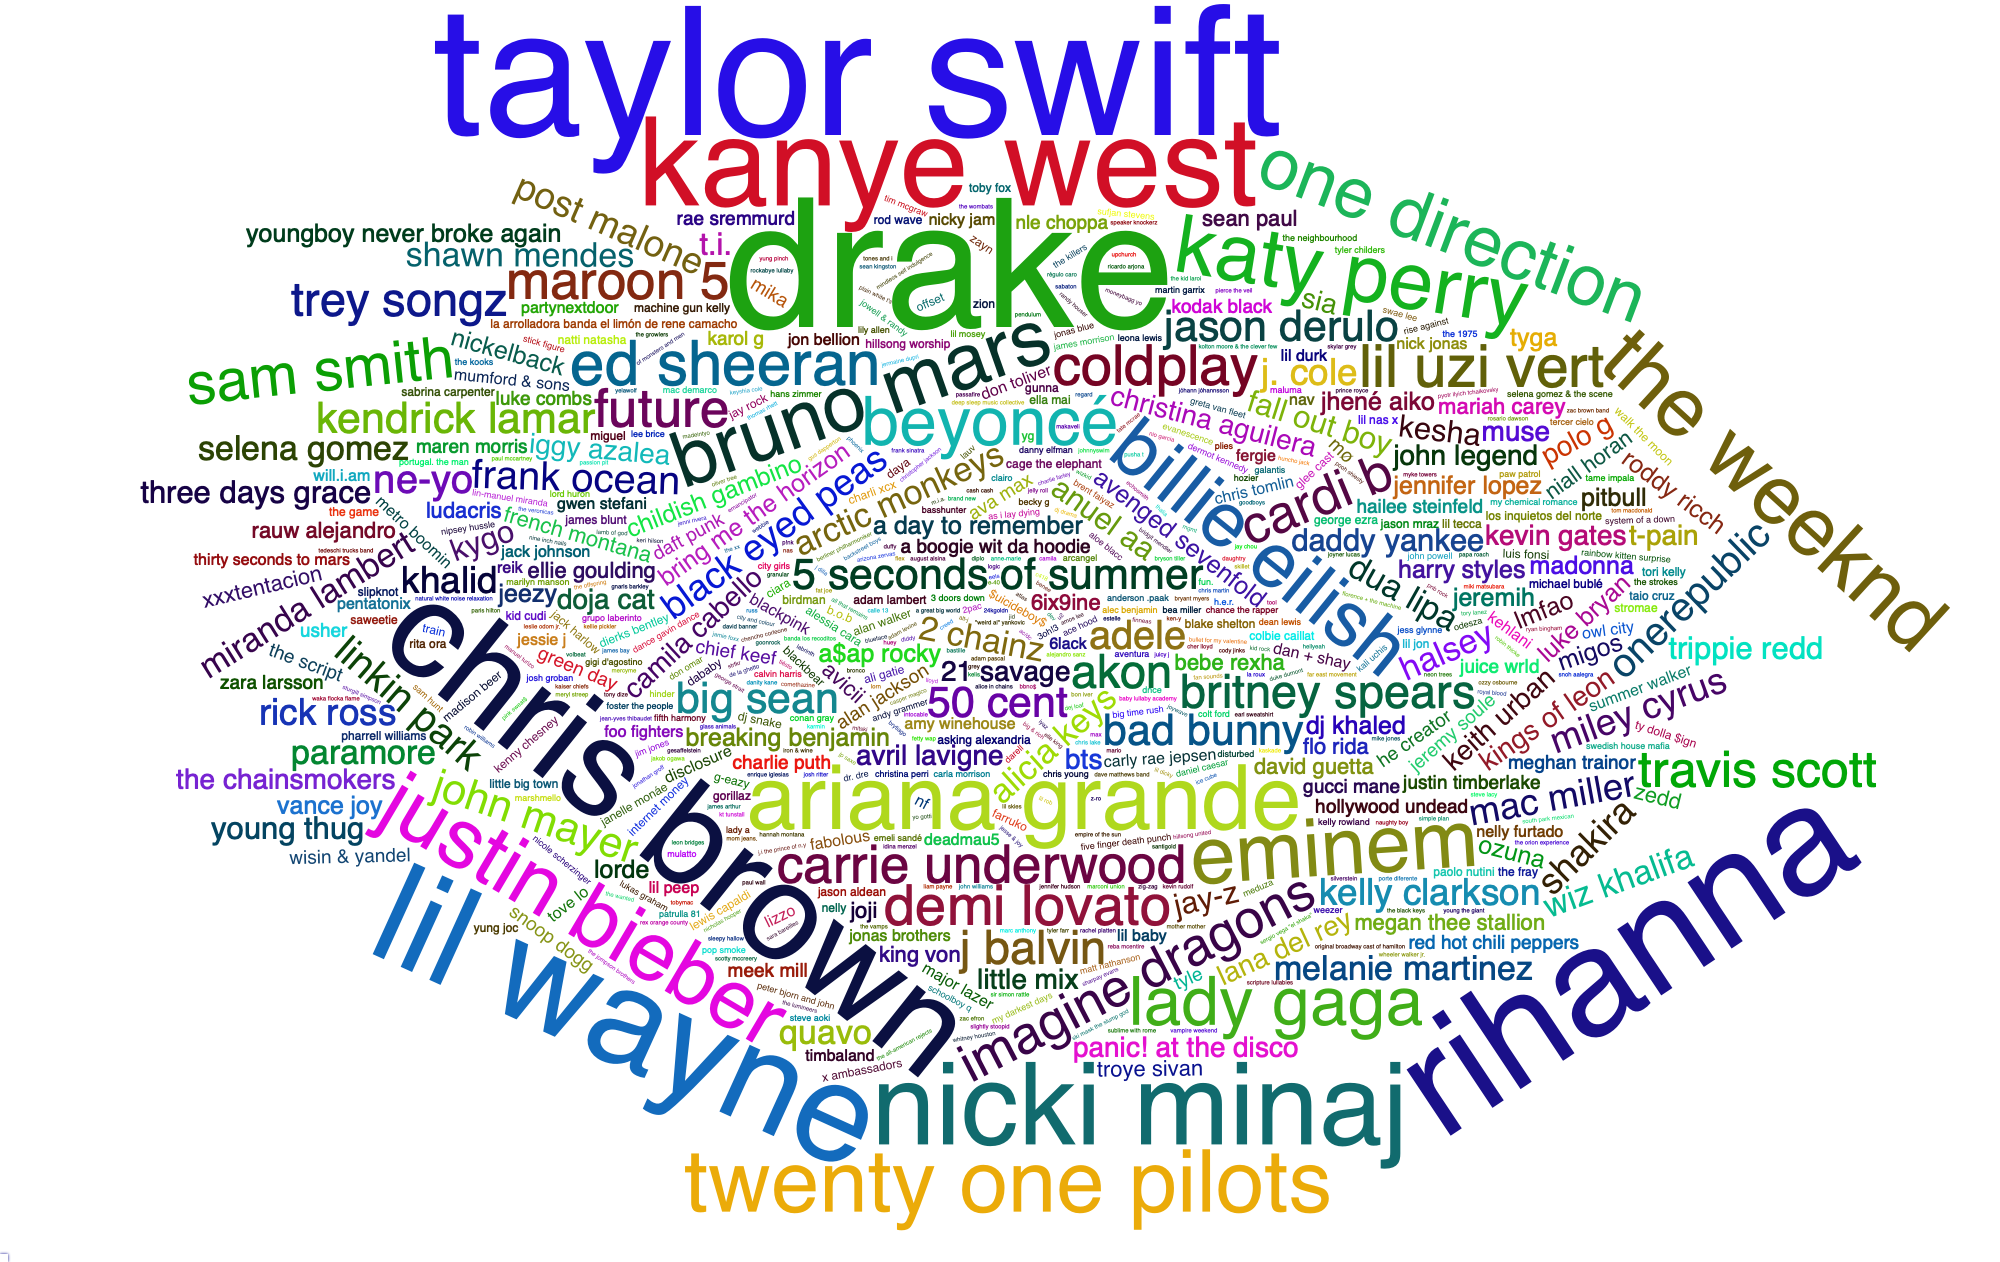
\includegraphics[width=14cm]{../images/wordcloud_overall_fix.png}
	\caption{Wordcloud artisti considerando entrambe le classi.}
\end{figure}

Viene quindi mostrato il worcloud degli artisti andando a considerare
solo le canzoni di successo:

\begin{figure}[H]
	\centering
	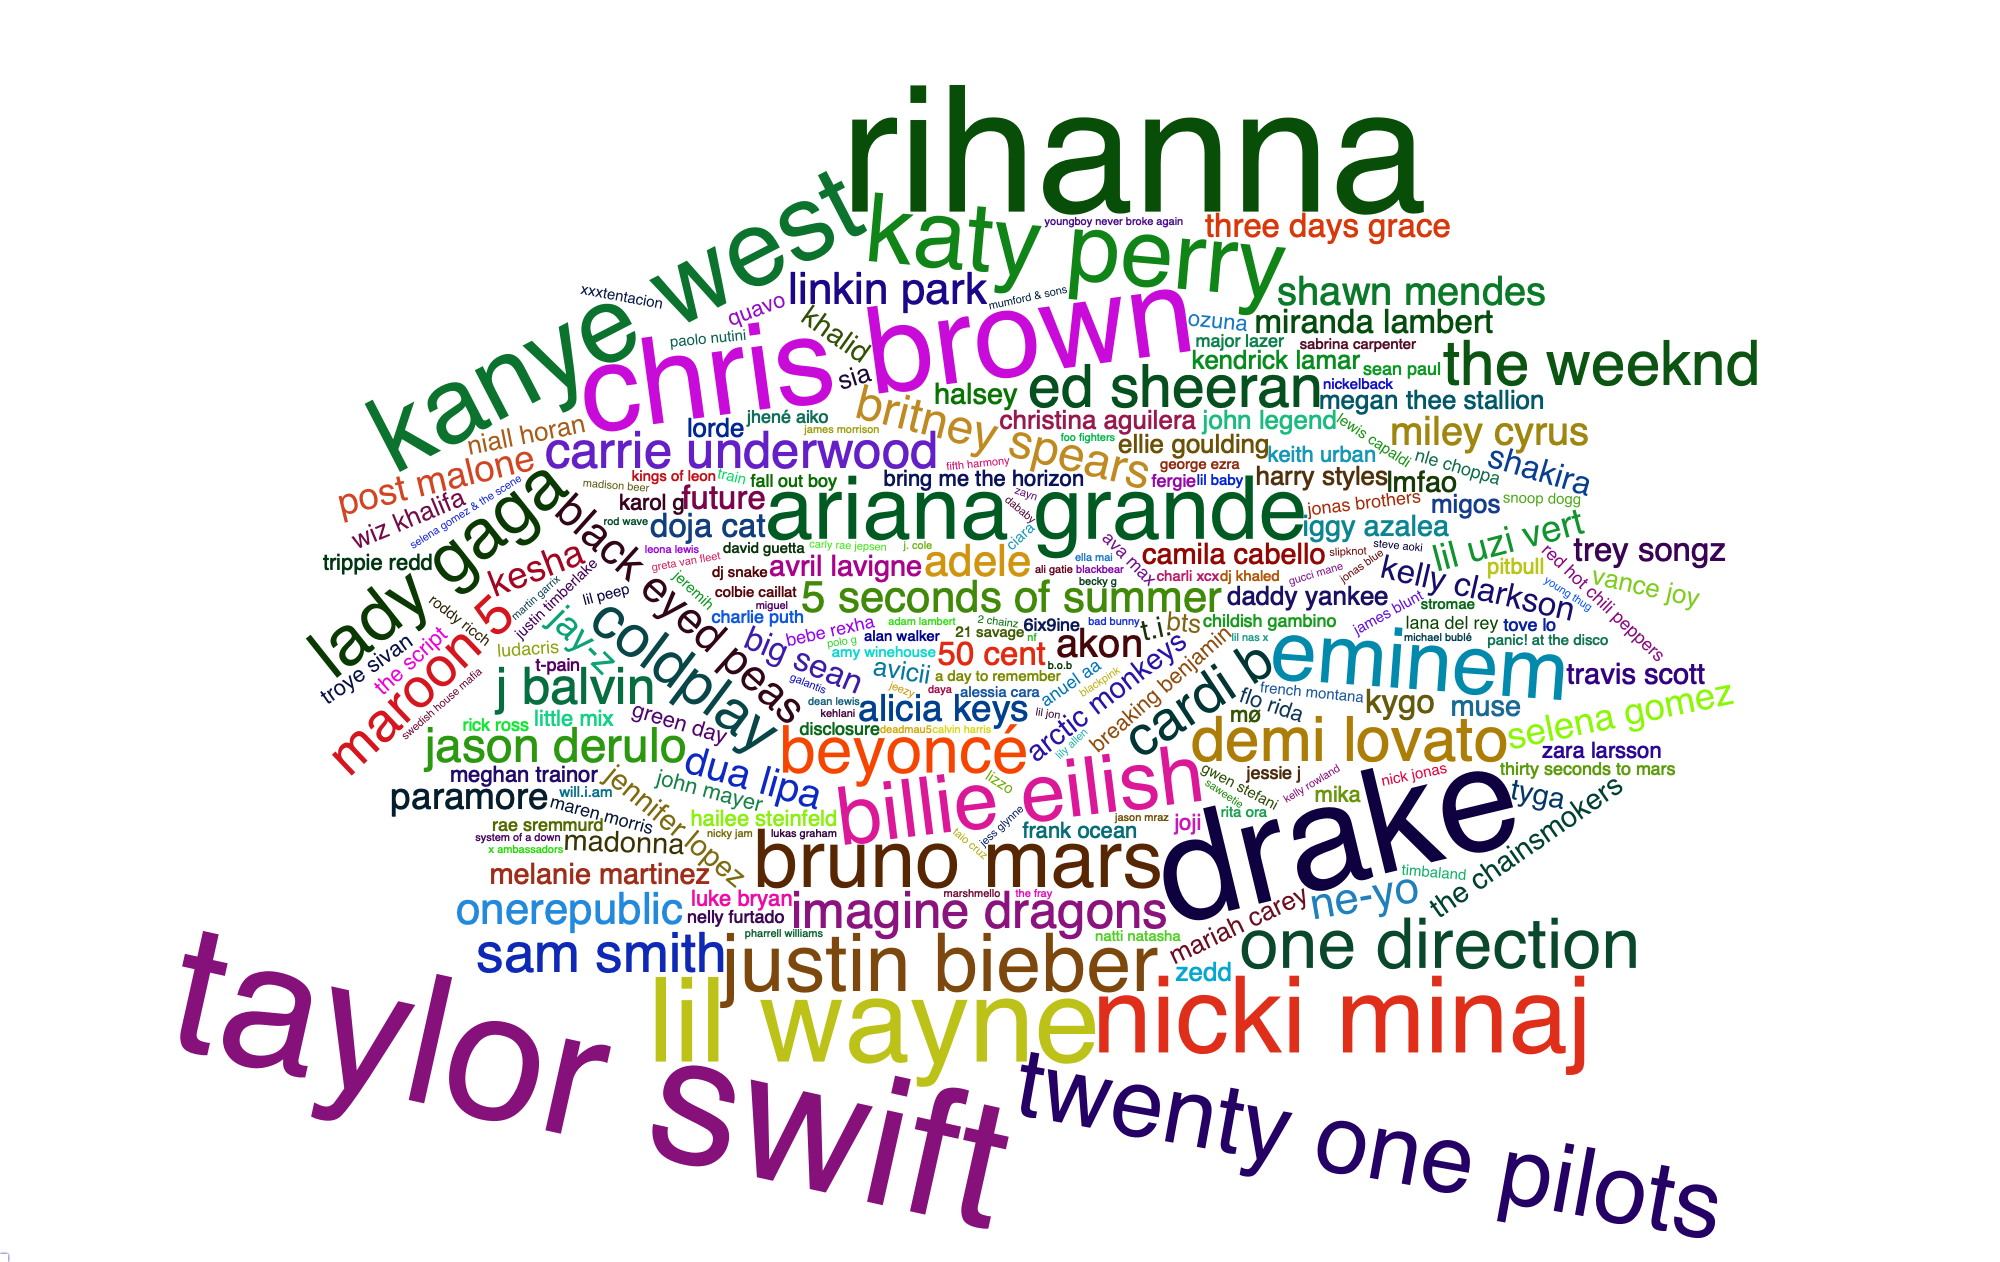
\includegraphics[width=14cm]{../images/wordcloud_positive_fix.png}
	\caption{Wordcloud artisti considerando solo la classe positiva.}
\end{figure}

Analogamente il worcloud degli artisti considerando solo le canzoni
non di successo:

\begin{figure}[H]
	\centering
	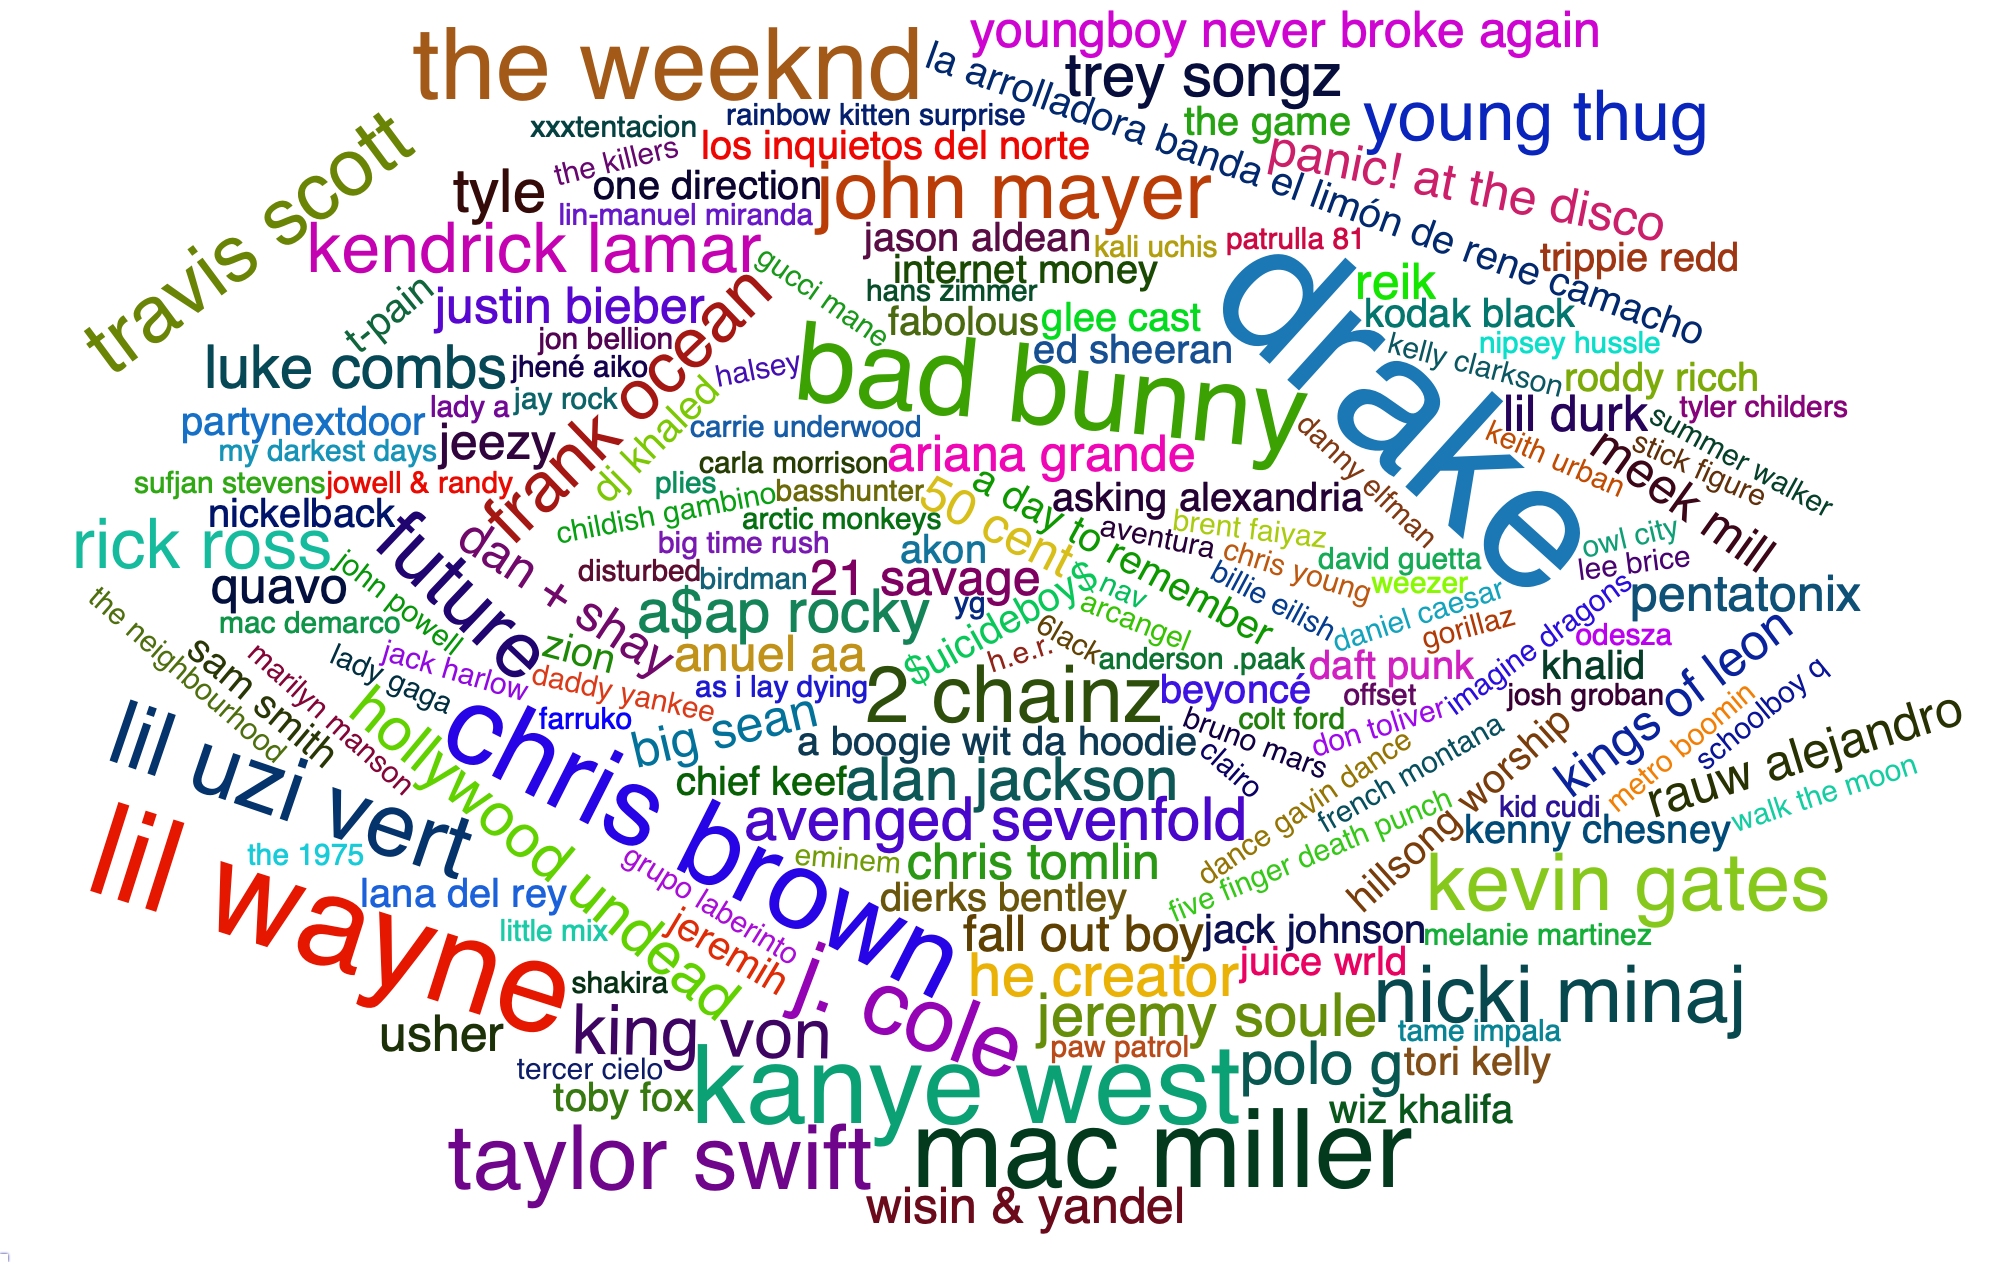
\includegraphics[width=14cm]{../images/wordcloud_negative_fix.png}
	\caption{Wordcloud artisti considerando solo la classe negativo.}
\end{figure}

Dai grafici emerge che molti artisti compaiono sia nella classe
positiva che in quella negativa. Tuttavia ci sono alcuni artisti
e.g. "Taylor Swift" o "Rihanna" che spiccano nella classe di successo
mentre sono meno frequenti nei brani non di successo. A fronte di
questa analisi riteniamo che considerare gli artisti all'interno di un
brano possa essere utile per distinguere le due classi. Viene quindi
utilizzata una rappresentazione one hot encoding (spiegato in
\autoref{sec:one}) per utilizzare questa informazione durante la fase
di training dei modelli.


\subsection{Correlazione tra features}
\label{sec:correlazione}
Si considera ora la correlazione tra le faetures numeriche. A questo
scopo calcoliamo la matrice di correlazione e la rappresentiamo qui
sotto per mezzo di una heatmap:

\begin{figure}[H]
	\centering
	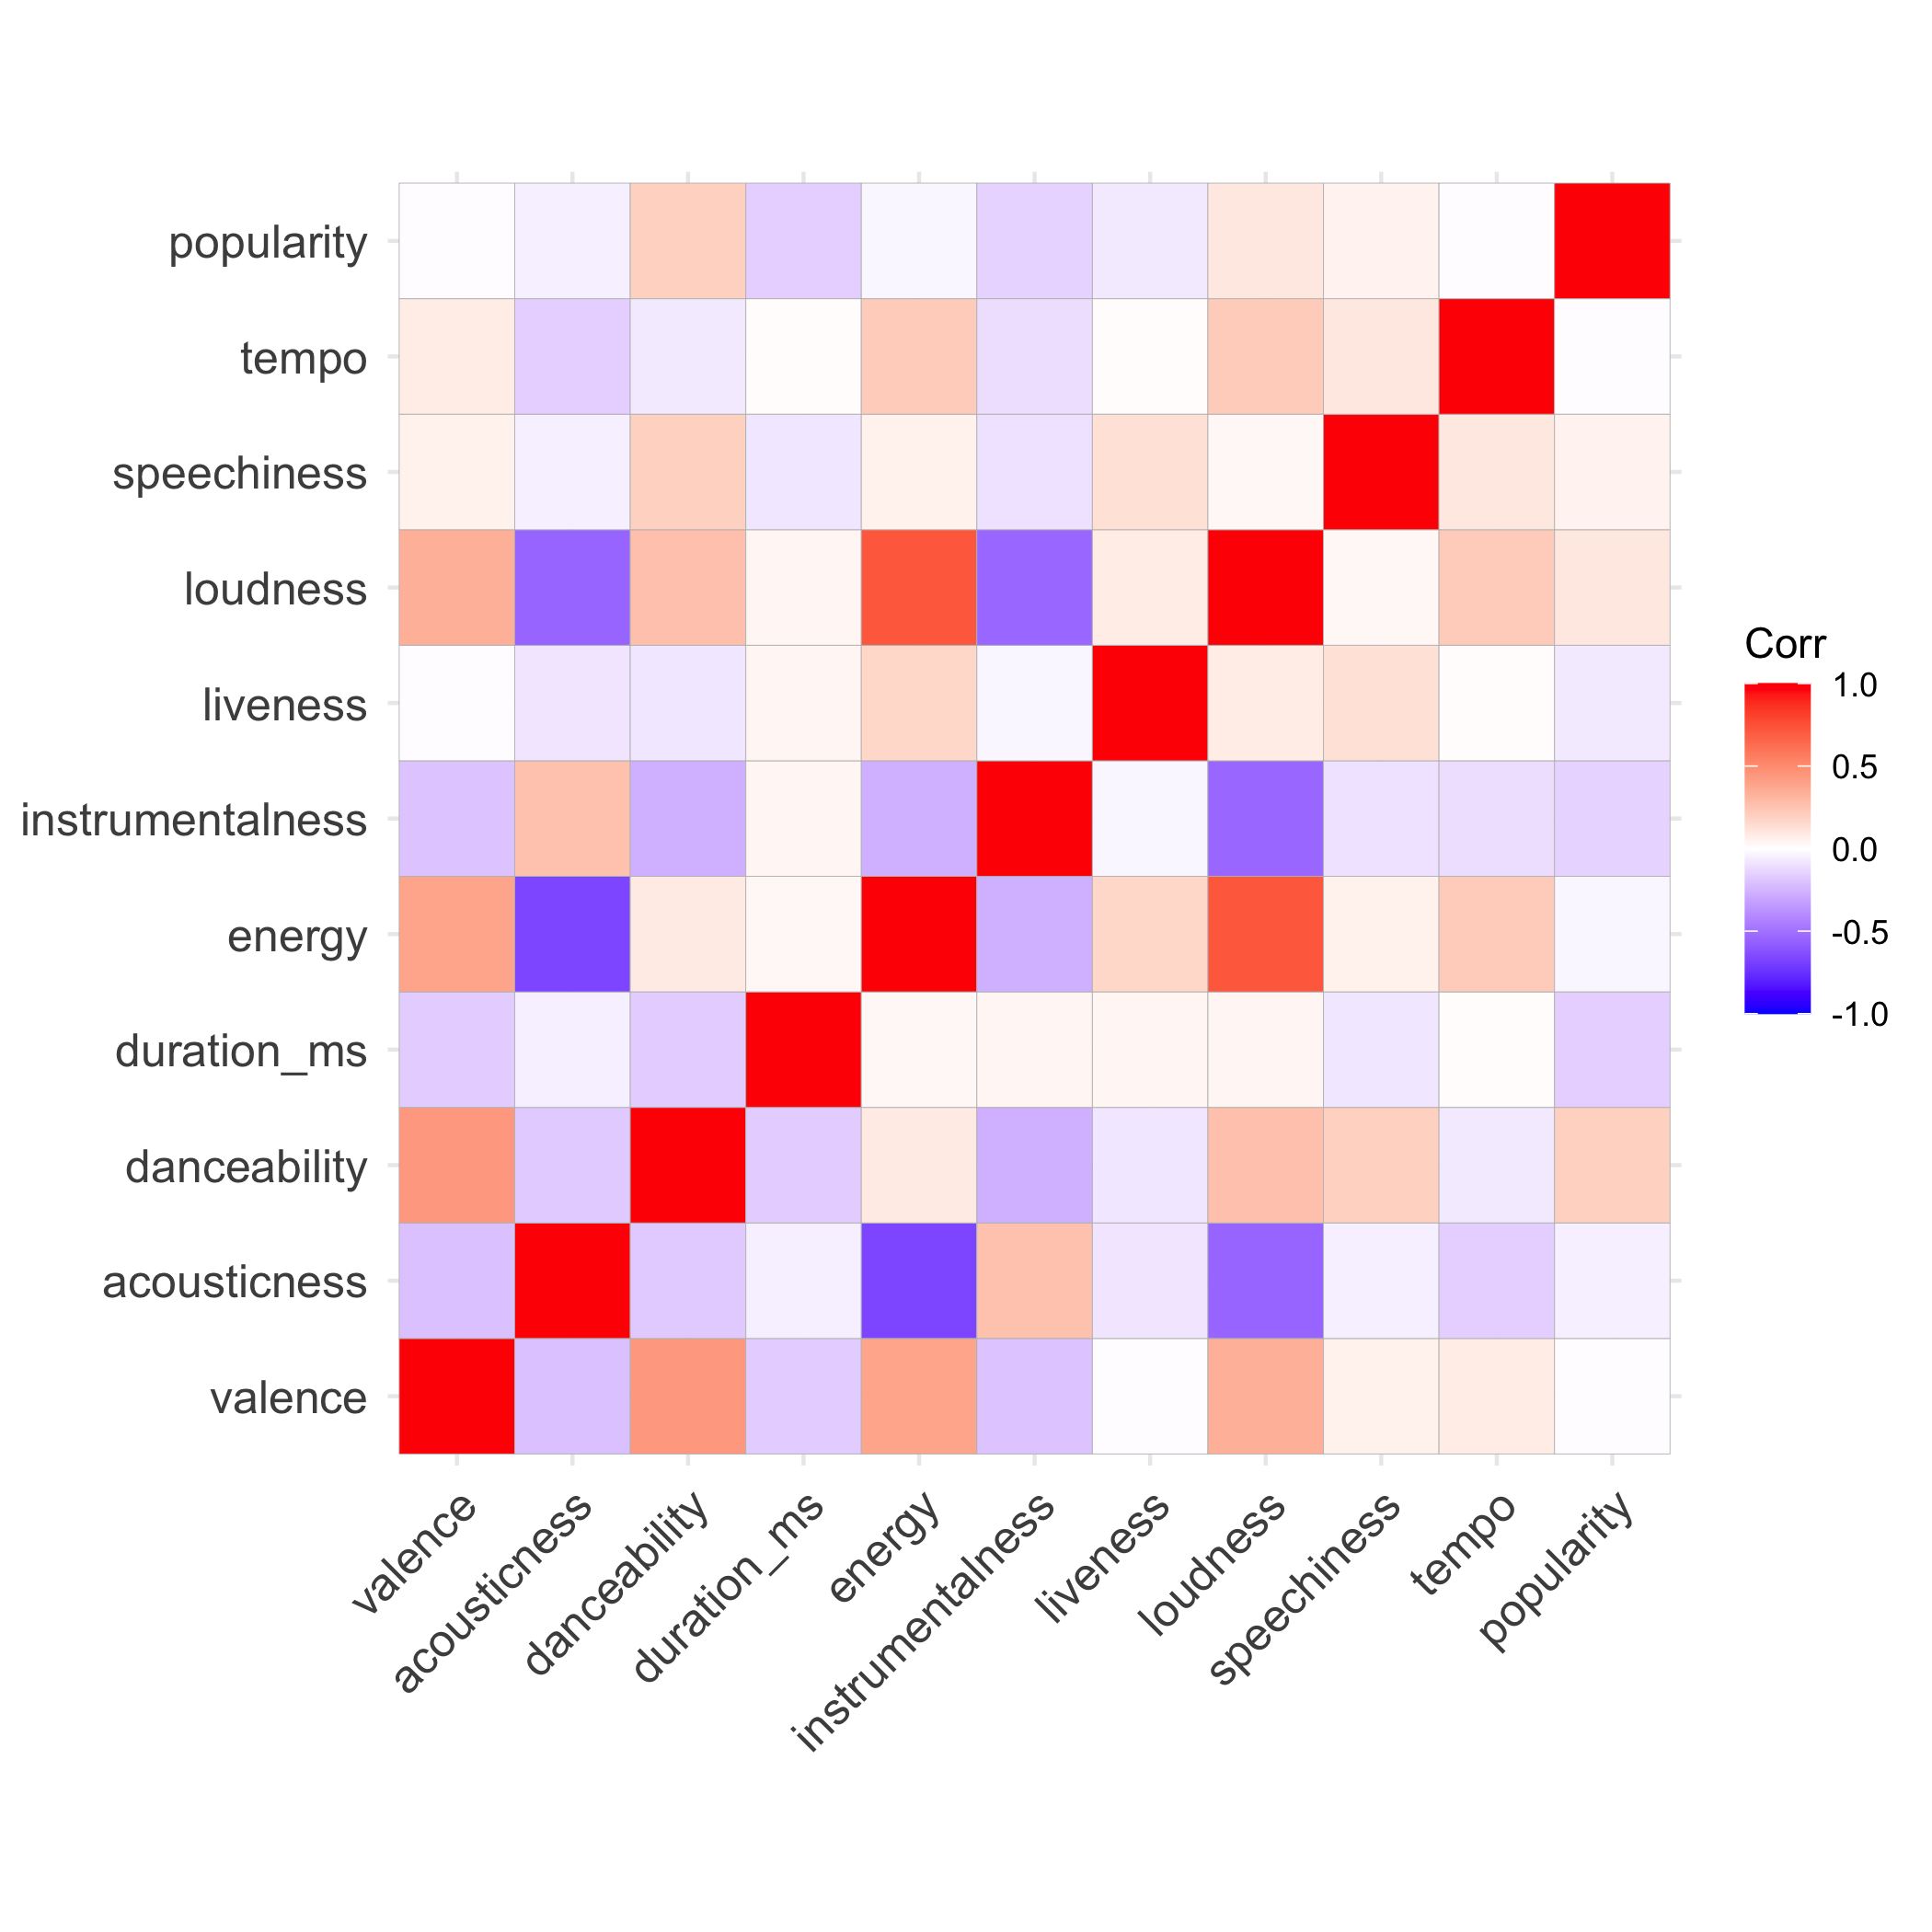
\includegraphics[width=14cm]{../images/correlation.png}
	\caption{Matrice di correlazione.}
\end{figure}

Da questa immagine si può notare come alcune covariate, ad esempio
"energy" e "loudness", sono correlate positivamente, mentre altre
covariate come "acousticness" e "energy" oppure "acousticness"e
"loudness" sono correlate negativamente. Questo rispecchia il senso
comune di energia di una canzone, e ci si aspetta che al crescere di
questa aumenta anche la loudness di un brano.

\subsection{Principal component analysis}
\label{sec:pca}
Dal momento che esiste correlazione tra le covariate, viene utilizzata
la tecnica PCA con lo scopo di ridurre la dimensione del dataset
spiegando la maggior parte della varianza.

La PCA viene effettuata solo sulle features numeriche, si noti inoltre
come il dataset è stato precedentemente standardizzato, in questo modo
i valori numerici hanno media $0$ e varianza $1$. Questa è
una condizione necessaria per applicare correttamente la tecnica PCA.

A partire dalla matrice di covarianza viene effettuata la
decomposizione agli autovalori, si ottengono quindi gli autovettori
con gli autovalori associati. Ordinando gli autovalori in ordine
decrescente viene mostrata la varianza spiegata da ogni componente
principale, oltre che alla varianza spiegata cumulata.

\begin{figure}[H]
	\centering
	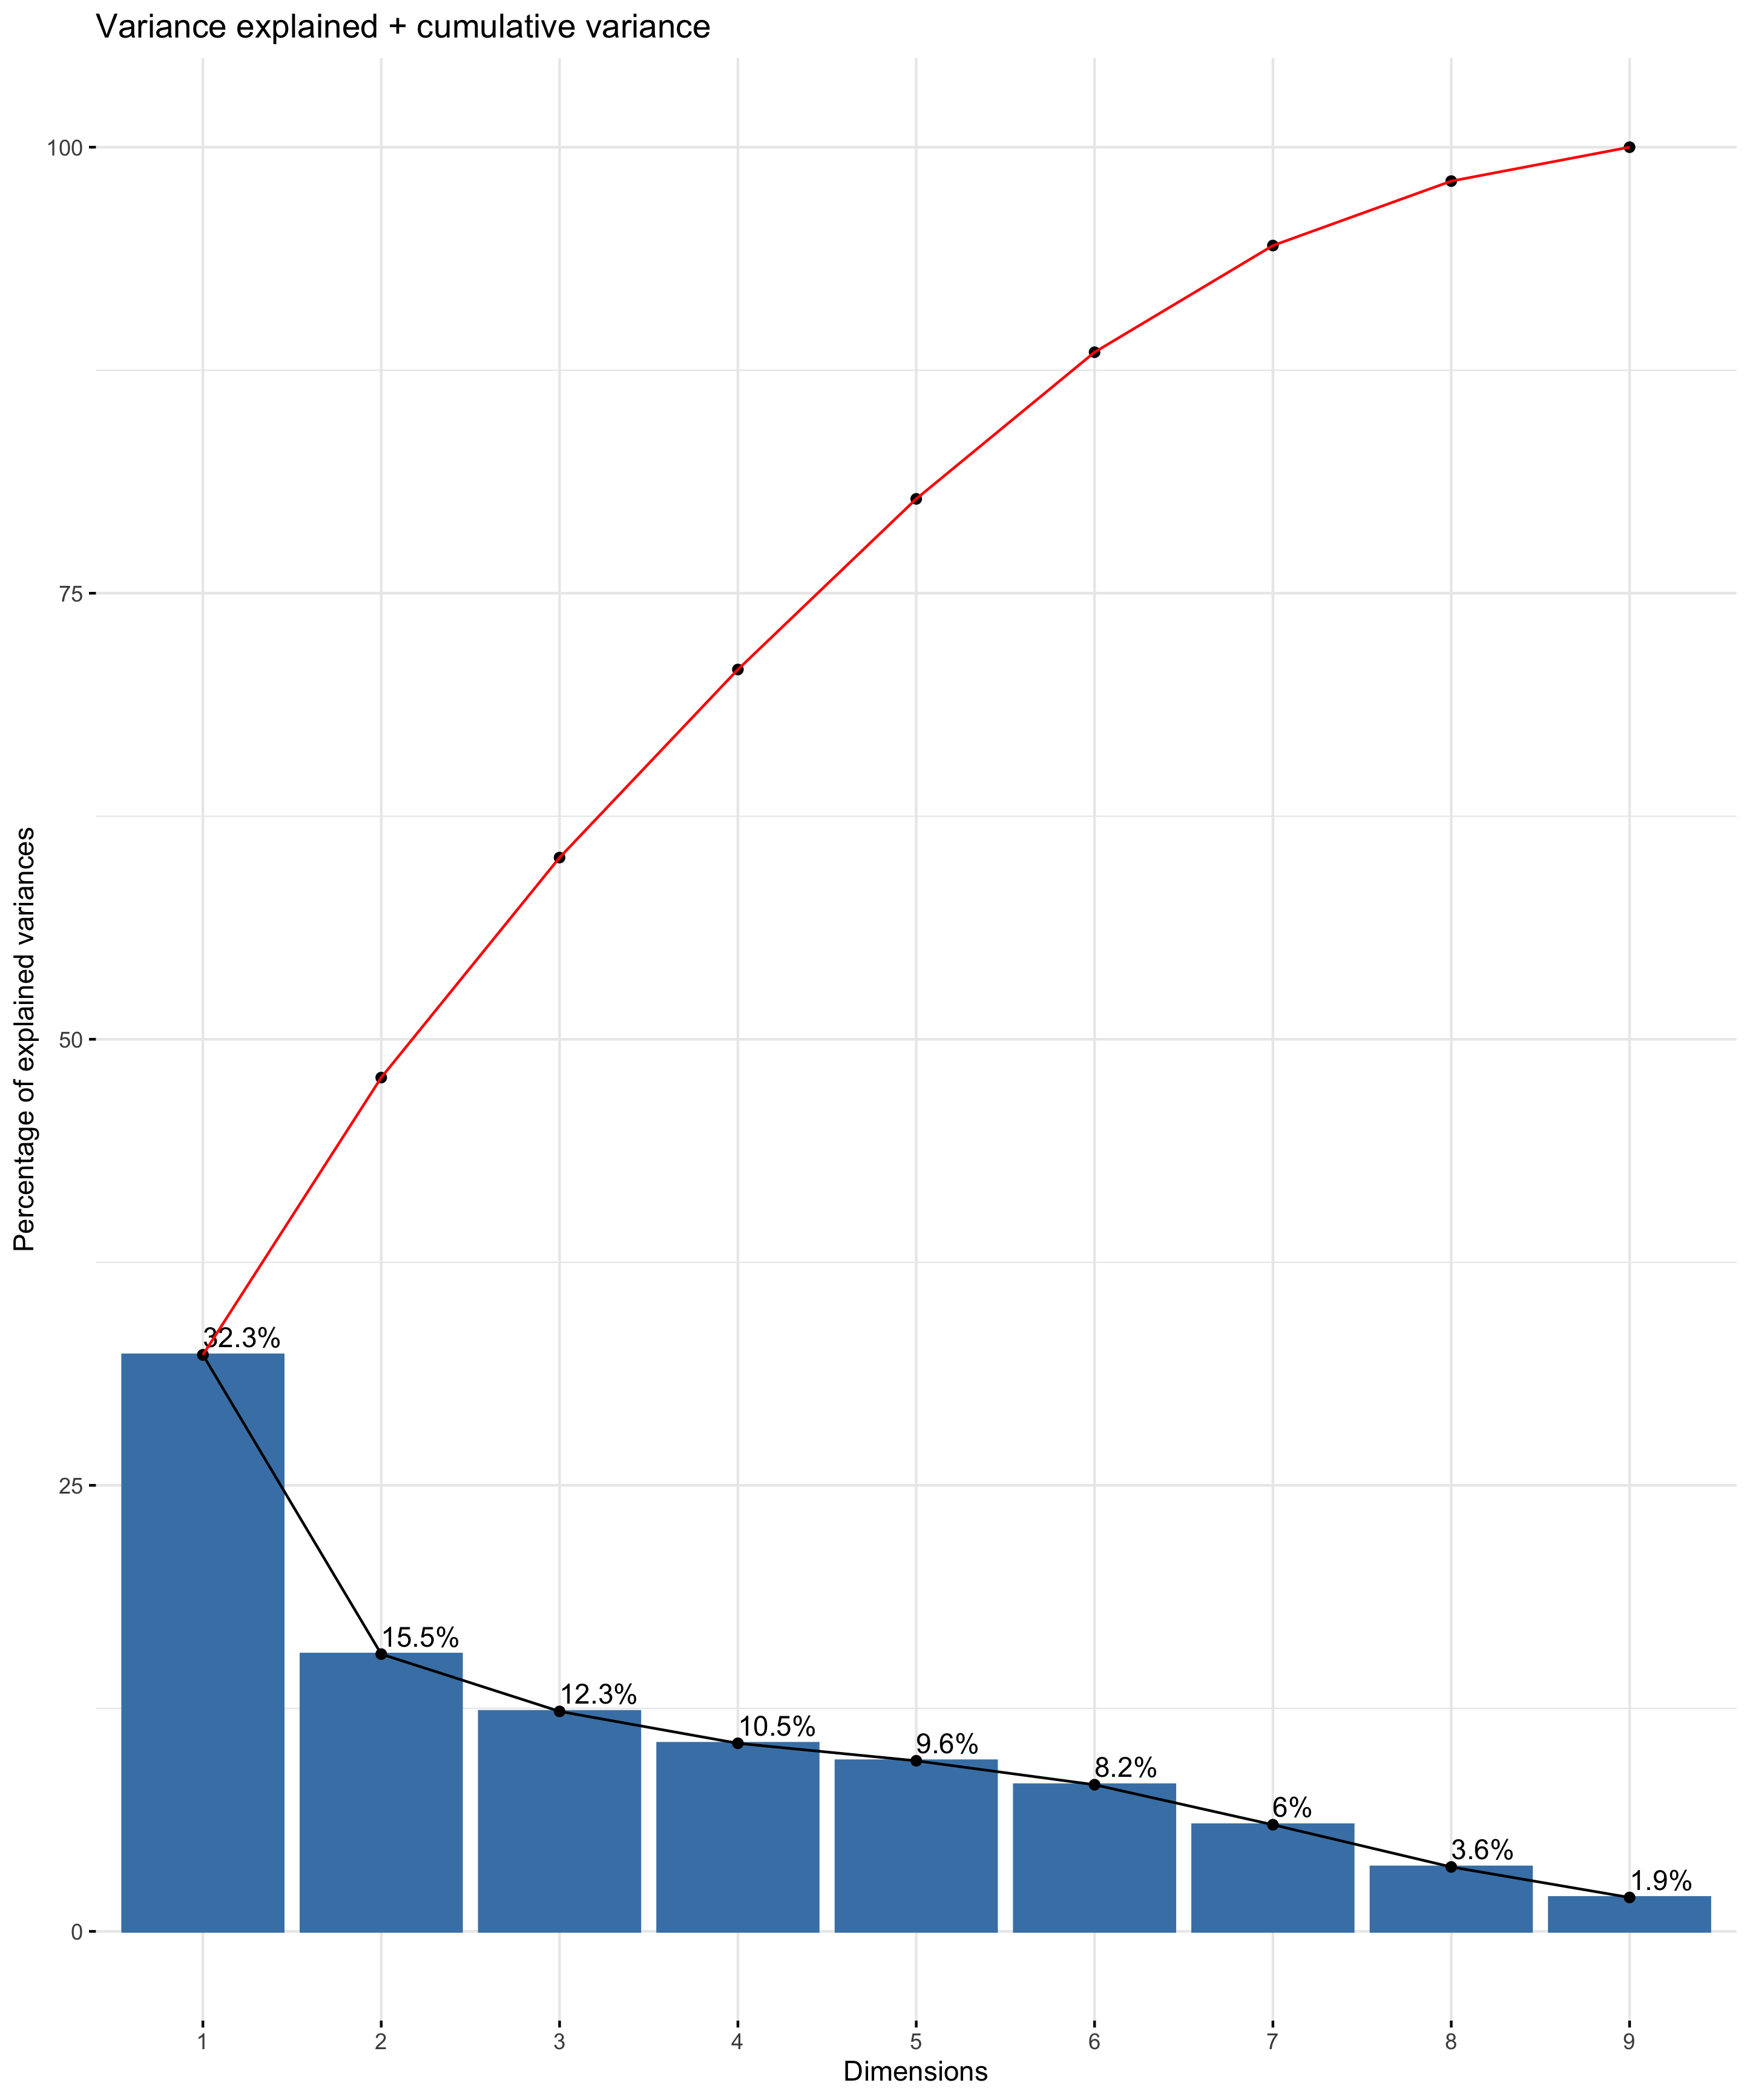
\includegraphics[width=13cm]{../images/pca_variance_explained.png}
	\caption{Varianza spiegata dalle componenti principali.}
\end{figure}

In tabella viene riportata la varianza spiegata cumulata:


	\begin{tabular}{|l c c c c c c c c c|} 
		\hline
		PC1 & PC2 & PC3 & PC4 & PC5 & PC6 & PC7 & PC8 & PC9 & PC10\\
		\hline
		29.72 &
		44.22 &
		55.39 &
		65.20 &
		74.33 &
		82.45 &
		89.58 &
		94.78 &
		98.26 &
		100.00 \\
		\hline
		
	\end{tabular}

Sulla base di questi dati è possibile notare come le prime $7$
componenti principali spiegano circa il $90\%$ della varianza
totale. Per questo motivo si sceglie di proiettare il dataset dallo
spazio originale nel nuovo sottospazio trovato con la PCA. Questo
nuovo spazio ha dimensione pari a $7$, ovvero il numero di componenti
principali che si è scelto di utilizzare.

\section{Scelta delle features}
In questa sezione viene spigata e giustificata la scelta di ogni
feature.

\subsection{Variabili scartate}
Come si può notare dalla \autoref{tab:features} non tutti le features
vengono utilizzate. Le variabili scartate sono le seguenti:

\begin{itemize}
	\item \textbf{id}: ID assegnato da spotify a ogni brano musicale. Questo campo non è rilevante per distinguere le due classi
	\item \textbf{name}: Titolo del brano musicale. Questa variabile non è utilizzata. Si potrebbero usare tecniche di NLP per tenere conto del sentiment del titolo brano e usare questa feature aggiuntiva.
	\item \textbf{release\_data}: 
	L'anno di rilascio del brano viene utilizzato solo per la fase iniziale per scartare i brani troppo vecchi. Questa covariata non viene utilizzata per il training in quanto si ritiene che non sia influente per distinguere le due classi (\autoref{fig:year_boxplot_award}). Inoltre si vogliono costruire modelli che siano indipendenti dalla data di rilascio.
	\item \textbf{year}: Campo uguale a "release\_date". Nel dataset questa informazione è duplicata. 
	\item \textbf{popularity}: Questo campo non viene utilizzato per i motivi discussi in \autoref{sec:popularity}
\end{itemize}


\subsection{Rappresentazione one hot encoding degli artisti}
\label{sec:one}
Dopo aver analizzato i wordcloud degli artisti emerge che questa
informazione è utile per distinguere le due classi. Si procede quindi
costruendo l'insieme degli artisti tra tutte le canzoni. Per ogni
artista viene tenuto traccia del numero di brani musicali in cui
l'artista compare.

La frequenza è necessaria perchè si vogliono tenere solo gli artisti
che hanno una frequenza maggiore o uguale a $2$. Questa operazione
viene effetuata per non contare gli artisti completamente sconosciuti,
in quanto si ritengono non influenti ai fine della classificazione.
Inoltre a causa dell'undersampling è possibile avere diverse canzoni
cantate da artisti "sconosciuti" e non avendo scelto una particolare
strategia per l'undersampling adottiamo a questo punto l'utilizzo di
un threshold.

Si procede quindi costruendo una matrice dove le colonne rappresentano
ogni artista nell'insieme degli artisti, le righe invece gli individui
nel dataset. L'entrata $i,\; j$ della matrice può contenere il valore
$1$ o $0$. Nel caso in cui il $j$-esimo artista ha cantanto nella
$i$-esima canzone allora l'entrata della matrice ha il valore $1$, $0$
altrimenti.

La matrice costruita costituisce la rappresentazione degli artisti
nelle canzoni.

\subsection{Variabili categoriche}
Tutte le variabile categoriche vengono utilizzate ai fini della
classificazione in quanto dalla descrizione della
\autoref{tab:features} risultano essere importanti nella distinzione
delle classi.

\subsubsection{Variabile key}
La variabile key è di tipo factor i cui valori sono numeri da 1 a
11. Questa covariata indica la scala musicale utilizzata nella
canzone. Dal momento che esiste una relazione d'ordine totale tra le
note musicali, infatti si parla di scala musicale, per questa
variabile viene effettuata l'operazione di cast a intero. Come secondo
passo i valori vengono scalati in modo tale da essere compresi tra $0$
e $1$.

\subsubsection{Variabile mode}
La variabile mode è binaria, viene utilizzata impostando a $1$ se vero
$0$ altrimenti.

\subsubsection{Variabile explicit}
Per la variabile explicit si procede analogamento a come fatto per la
covariata mode.

\subsection{Coordinate PCA}
Le variabili numeriche non vengono direttamente usate per il training,
piuttosto si utilizza il nuovo spazio ottenuto dalla PCA. Questo nuovo
spazio ha dimensione inferiore rispetto al numero di variabili
numeriche iniziale, ed è stato costruito proiettando gli individui del
dataset di partenza nel nuovo spazio che ha come basi le $7$
componenti principali.

\subsection{Riassunto feature finali utilizzate}


\begin{table}[H]
	
	\begin{center}
		
		\begin{tabular}{ |l|c| }
			\hline
			\multicolumn{1}{ |c }{\textbf{FEATURE}} &
			\multicolumn{1}{ c |}{\textbf{\# COVARIATE}} \\
			\hline
			\hline
			One-hot-encoding artisti & 
			$655$\\
			Componenti principali & 
			$7$\\
			Variabili categoriche & 
			$3$\\
			Label & 
			$1$\\
			\hline
			
			\multicolumn{1}{ c }{ } &
			\multicolumn{1}{ | c |}{666} \\
			\cline{2-2}
			
		\end{tabular}
		
	\end{center}
	\caption{Tabella riassuntiva features utilizzate.}
\end{table}
